% 导言区
\documentclass[a4paper, UTF8]{article}
\pdfpagewidth=15.5in
\pdfpageheight=20in

\usepackage{ctex}
\usepackage{geometry}

\geometry{left = 3.0cm,right = 3.0cm,top = 2.0cm,bottom = 2.0cm}
\usepackage{times}
\usepackage{soul}

\usepackage{indentfirst} 
%\usepackage[CJKbookmarks]{hyperref}
\usepackage[encapsulated]{CJK}

\usepackage{url}
\usepackage[hidelinks]{hyperref}


\usepackage{algorithm}  
\usepackage{algorithmicx}
\usepackage{algpseudocode}  
\usepackage{amsmath}  
\renewcommand{\algorithmicrequire}{\textbf{Input:}}  
\renewcommand{\algorithmicensure}{\textbf{Output:}}  


\usepackage[utf8]{inputenc}
\usepackage[small]{caption}

\usepackage{graphicx}
\usepackage{wrapfig}
\usepackage{subfigure}
\usepackage{booktabs}
\usepackage{amsthm,amsmath,amssymb}

\usepackage{mathrsfs}
%\usepackage{algorithmic}
\urlstyle{same}

\newtheorem{example}{Example}
\newtheorem{theorem}{Theorem}


\newcommand{\name}{\kaishu 城市整体异常检测}

\title{
	\begin{figure}[ht]
	%\centerline{
\includegraphics[scale = 1]{hit.jpg}}
	
\includegraphics[scale = 1]{hit.jpg}
	\centering
	\end{figure}
	\begin{center}
	\Large{\kaishu 大数据计算基础课程报告}
	\end{center}
	\textbf{\name}\\
}
\author{
	\textbf{专业:大数据专业}\\
	\textbf{学号:1173710224}\\
	\textbf{姓名:陈泊舟}\\
	\textbf{课程:大数据计算基础}\\
}




\makeatletter
\newenvironment{breakablealgorithm}
  {% \begin{breakablealgorithm}
   \begin{center}
     \refstepcounter{algorithm}% New algorithm
     \hrule height.8pt depth0pt \kern2pt% \@fs@pre for \@fs@ruled
     \renewcommand{\caption}[2][\relax]{% Make a new \caption
       {\raggedright\textbf{\ALG@name~\thealgorithm} ##2\par}%
       \ifx\relax##1\relax % #1 is \relax
         \addcontentsline{loa}{algorithm}{\protect\numberline{\thealgorithm}##2}%
       \else % #1 is not \relax
         \addcontentsline{loa}{algorithm}{\protect\numberline{\thealgorithm}##1}%
       \fi
       \kern2pt\hrule\kern2pt
     }
  }{% \end{breakablealgorithm}
     \kern2pt\hrule\relax% \@fs@post for \@fs@ruled
   \end{center}
  }
\makeatother




\begin{document}
\begin{CJK}{UTF8}{gbsn}
\maketitle
\newpage
\CJKindent
\begin{abstract}
整体异常检测指的是一个附近地点的集合在几个连续的时间段内由多个数据集共同识别的现象。整体异常表明存在潜在的问题,可能无法基于单个数据源或单一地点得出。通过关联多个地点和不同数据集,可以形成对事件的全景描述和检测。通过这样的方法,可以检测出以往的方法无法检测的异常,具有较强的应用背景和实际意义。近十年来异常检测问题受到研究人员的广泛关注,从单一数据集到跨越数据集,再到考虑跨越地区的影响因素,系统的异常检测能力越来越强。但是到目前为止所有的研究工作都在一个固定的时间段内部展开的,并且对于流量分布的拟合也不尽合理,没有充分利用大量的历史数据,除此之外还不具有时效性。针对这些问题我提出了一种实时的整体异常检测系统:我将时间维度纳入考虑,并且分析了拟合流量的更好的方法,成功地将问题抽象成一个基于历史数据的、自适应的超参数优化模型,并且为其设计大数据实时计算方法,从而实现从批处理到实时处理的转变。在使用时系统由四个模块构成:基于$MapReduce$的数据处理模块,基于神经网络的预测模块,跨越多个数据集以及地区的异常度计算模块,基于异常覆盖范围的异常分类模块。我使用了来自纽约市开源数据平台的多个源数据集训练并评估本系统:311 complaints, taxicab data等。实验表明,该方法优于对照组中的七种方法,表现很好。\\
\textbf{关键词}:整体异常,$MapReduce$,神经网络,贝叶斯优化,跨时间,跨区域,跨数据集
\end{abstract}
\tableofcontents


\section{绪论}
\subsection{研究问题的背景}
\ 传感技术和大规模计算基础设施的进步产生了各种各样的城市数据,例如交通流、人的流动性和社会媒体。这些数据集通常与时空信息相关。当它们一起存放时就可以代表城市的动态和节奏。按照前人的工作,整体异常分为两个类别,一个是考虑在一段时间内跨越多个数据集产生异常,针对这一种检测,一般是发现潜在的尚未发展起来的危害,另一个是在一段时间内跨越多个地区产生异常,但是仅仅通过一个地区的数据却没有办法检测出来。如图\ref{m-dataset}所示,三个图片分别展示了不同的数据集对异常的表现,并且在每一张图片中都有异常的中央区域与周边区域的交互信息。
\begin{figure}[ht]
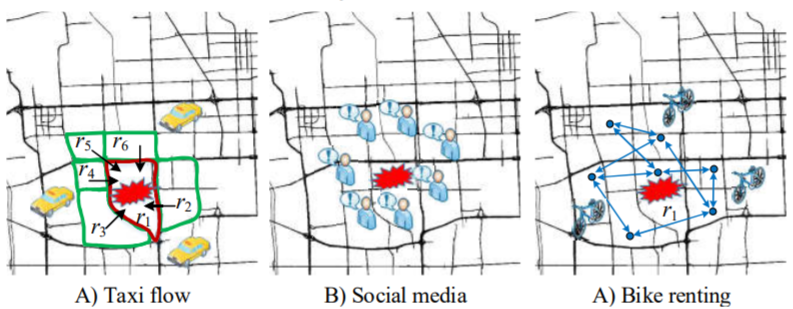
\includegraphics[scale = 0.9]{m-dataset.png}
\centering
\caption{整体异常跨数据集跨地区影响}
\label{m-dataset}
\end{figure}
\subsection{研究问题的挑战}
\ 为了进行城市整体异常的检测,有三个具有挑战性的问题需要解决:第一个是数据集信息的整合,比如数据集中哪些信息是有用的,有些数据集稀疏,有些数据集稠密,如何对不同格式的数据集进行基于$MapReduce$的统一的处理;第二个是数据集分布的拟合以及异常度的确定,在进行拟合时,数据集可能服从多种分布,也有可能在不同的时段服从不同的分布,如何进行统一的处理,并在拟合分布的基础上进行异常度的计算;第三个是信息的合并,这一点主要是跨数据集和跨地区的信息合并。
\subsection{当前工作的不足之处}
参考了上海交通大学2015年的一篇论文\cite{DalzielDetecting}(以下简称论文),论文针对数据集的稠密以及分布不同等多个问题给出了自己的解决办法。整体的思路即假设$311 complait$数据集中的数据服从高斯分布,车流数据服从的是泊松分布。使用$\kappa ^ 2$检验检测异常,再采用加权平方和的方法实现跨数据集的异常检测。
\par论文中一个不合理的假设就是数据集服从某个分布,如图\ref{figure1}所示,按照半个小时划分,一天分为48个时段,图1中显示的是某天出租车人流流入量随时间变化,从图中可以看出在某个时段服从高斯分布,但是也不是较为标准的分布模型,如果按照高斯分布进行检验,计算出的异常度就会很大。换言之,论文解决了整体异常的检测问题,但是检测的太过于宽泛,从而带来不必要的麻烦。其次,论文中并没有考量跨时间的影响因素,这使得有一些异常无法被判断出来。最后一个问题就是关于跨地区的解决办法,这将会在下面的章节中进行介绍。
\begin{figure}[ht]
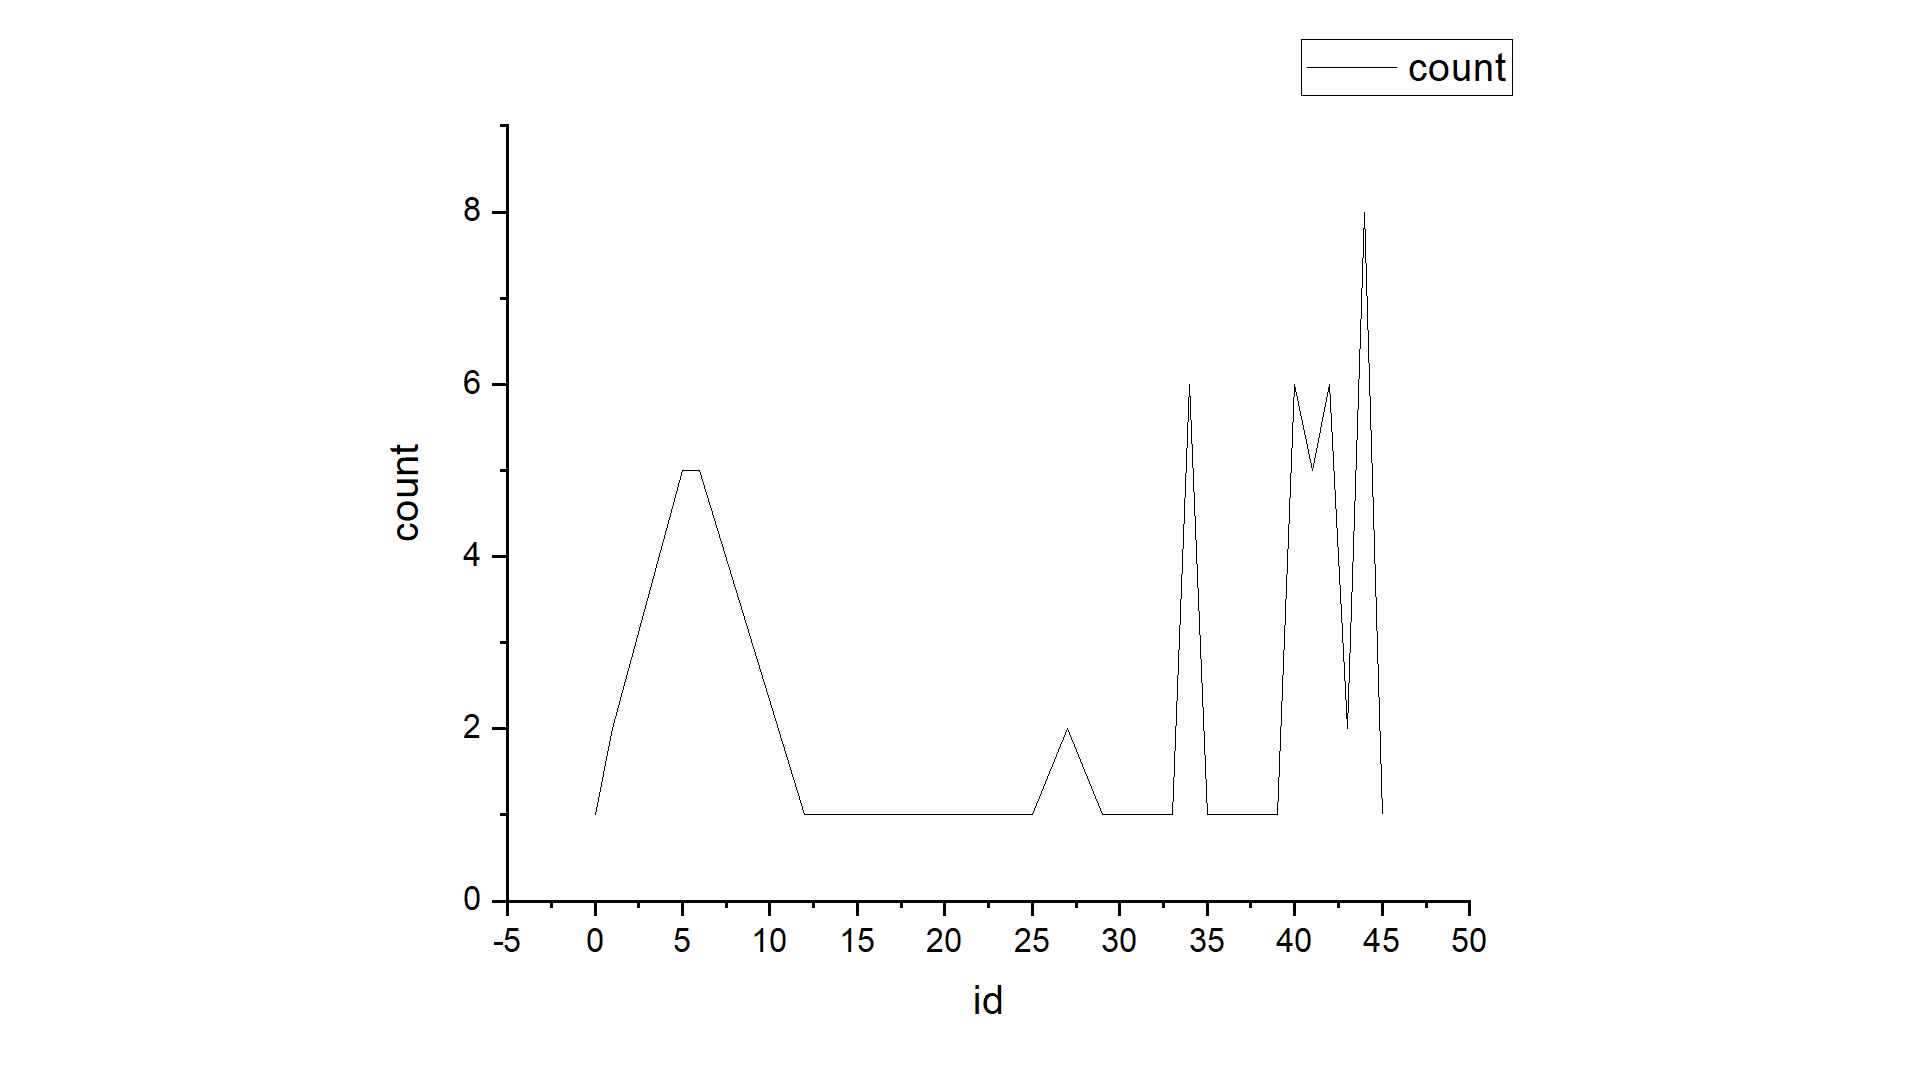
\includegraphics[scale = 0.3]{flow.png}
\centering
\caption{2014/6/20-229号区域出租车载客流入量随时间变化}
\label{figure1}
\end{figure}
\subsection{本文贡献}
本系统的贡献主要有四个。第一,提取数据集的分布特征,一个比较合适的方法是使用插值进行拟合,在本系统中使用神经网络进行拟合,考虑到每一个地区的差异性以及不同数据集的差异,每个地区每个数据集使用一个单独的神经网络拟合。第二,在$NN$拟合的基础之上进行异常度计算,将时间因素考虑在内,进行跨数据集、跨地区异常度计算,设计异常判断算法。第三,设计分类算法,对异常级别分类。第四,设计实现$MapReduce$接口程序,并且使系统能在大数据实时处理框架上运行。
\subsection{本文主要解决的问题以及方法}
\subsubsection*{数据整合}
在数据能够参与运算之前,需要做很多的处理,完成一定的格式转化。这部分工作的串行处理时间开销很大,但是处理是重复的、可并行的,因此可以设计基于$MapReduce$的并行处理方案。最终完成从$<\mathcal{D},l_x,l_y,C>$到$<r,\mathcal{D},s,C^{'}>$的转换。其中$\mathcal{D}$指的是日期,统一采用$\%Y-\%m-\%d\ \%H:\%M:\%S$的格式,$l_x,l_y$指的是事件发生的经纬度,$C$对于$311$数据集来讲是事件的类型,对于流数据集来讲是载客量,$r$为将经纬度映射到区域对应的编号,$s$为将一天划分为48个时段分别编号,并将日期中的24时映射到时段上,最后$C^{'}$对于$311$数据集指的就是在该区域该时间段发生的事件列表,对于$flow$数据集来说就是在该区域该时间段客流量。
\subsubsection*{数据分布拟合}
前面已经提到过,假设数据服从某一分布是不严谨的。考虑到后面的异常估计问题,在此采用神经网络(简称NN)进行拟合。由于不同地区不同数据集有不同分布,因而要使用不同的NN进行拟合。记作$NN(r,type)$,其中$r$表示区域编号,第二个参数表示所拟合数据集名字,$type \in ['311','bikeinflow','bikeoutflow','taxiinflow','taxioutflow']$。
	\subsubsection*{异常度估计}
针对每一个地区给出一个异常度,计算分为三个阶段:综合此前24小时的异常信息计算单个数据集的异常度,跨数据集的信息合并,跨地区的信息合并。计算公式为$across\_region$-$(\sqrt{\frac{\sum_{i}{w_i * ag_i} ^ {2} + {sign * ag_{311}} ^ {2}}{m}})$,在系统环节会详细解释三个计算过程。
	\subsubsection*{超参数优化}
在模型建立过程中引入了一些变量,比如在上一个小节给出的公式中,$w_i$就是一组超参数,另外在计算出异常度之后还要对异常进行判定,需要设定一组阈值,这也是超参数。经过统计,本系统总共有53个超参数需要标定。在本模型中采用基于$TPE$的贝叶斯优化方法进行超参数的调优。
\subsection{数据}
本次实验总共使用了关于纽约市的$5$个数据集,他们分别是:311 complaints, taxicab data, bike rental data, points of interest, and road network data。在系统的训练中主要使用的是311,taxi,bi-ke数据集,并将其转化成$311.csv$,$bikeinflow.csv$,$bikeoutflow.csv$,$taxiinflow.csv$,taxioutflow.-csv数据集进行使用。
\begin{figure}[ht]
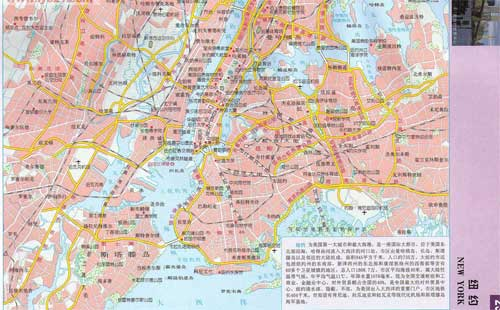
\includegraphics[scale = 0.4]{nyc.jpg}
\centering
\caption{纽约市地图}
\label{nyc}
\end{figure}
\subsubsection*{region}
第一个数据集是$NYC\_862.txt$。数据集将(40.918$^{\circ}$N, -74.259 $^{\circ}$E, 40.486$^{\circ}$N, -73.7$^{\circ}$E)之间的区域划分为2400 * 2400的矩阵,任何一个经纬度表示的坐标点都可以映射到矩阵中的一个小单元上。矩阵中的每一个小单元上都有一个数字,这个数字代表的是它属于哪个区域,单元编号相同的属于同一个区域,如果编号是0,代表这个小单元不属于任何一个区域。
\begin{figure}[ht]
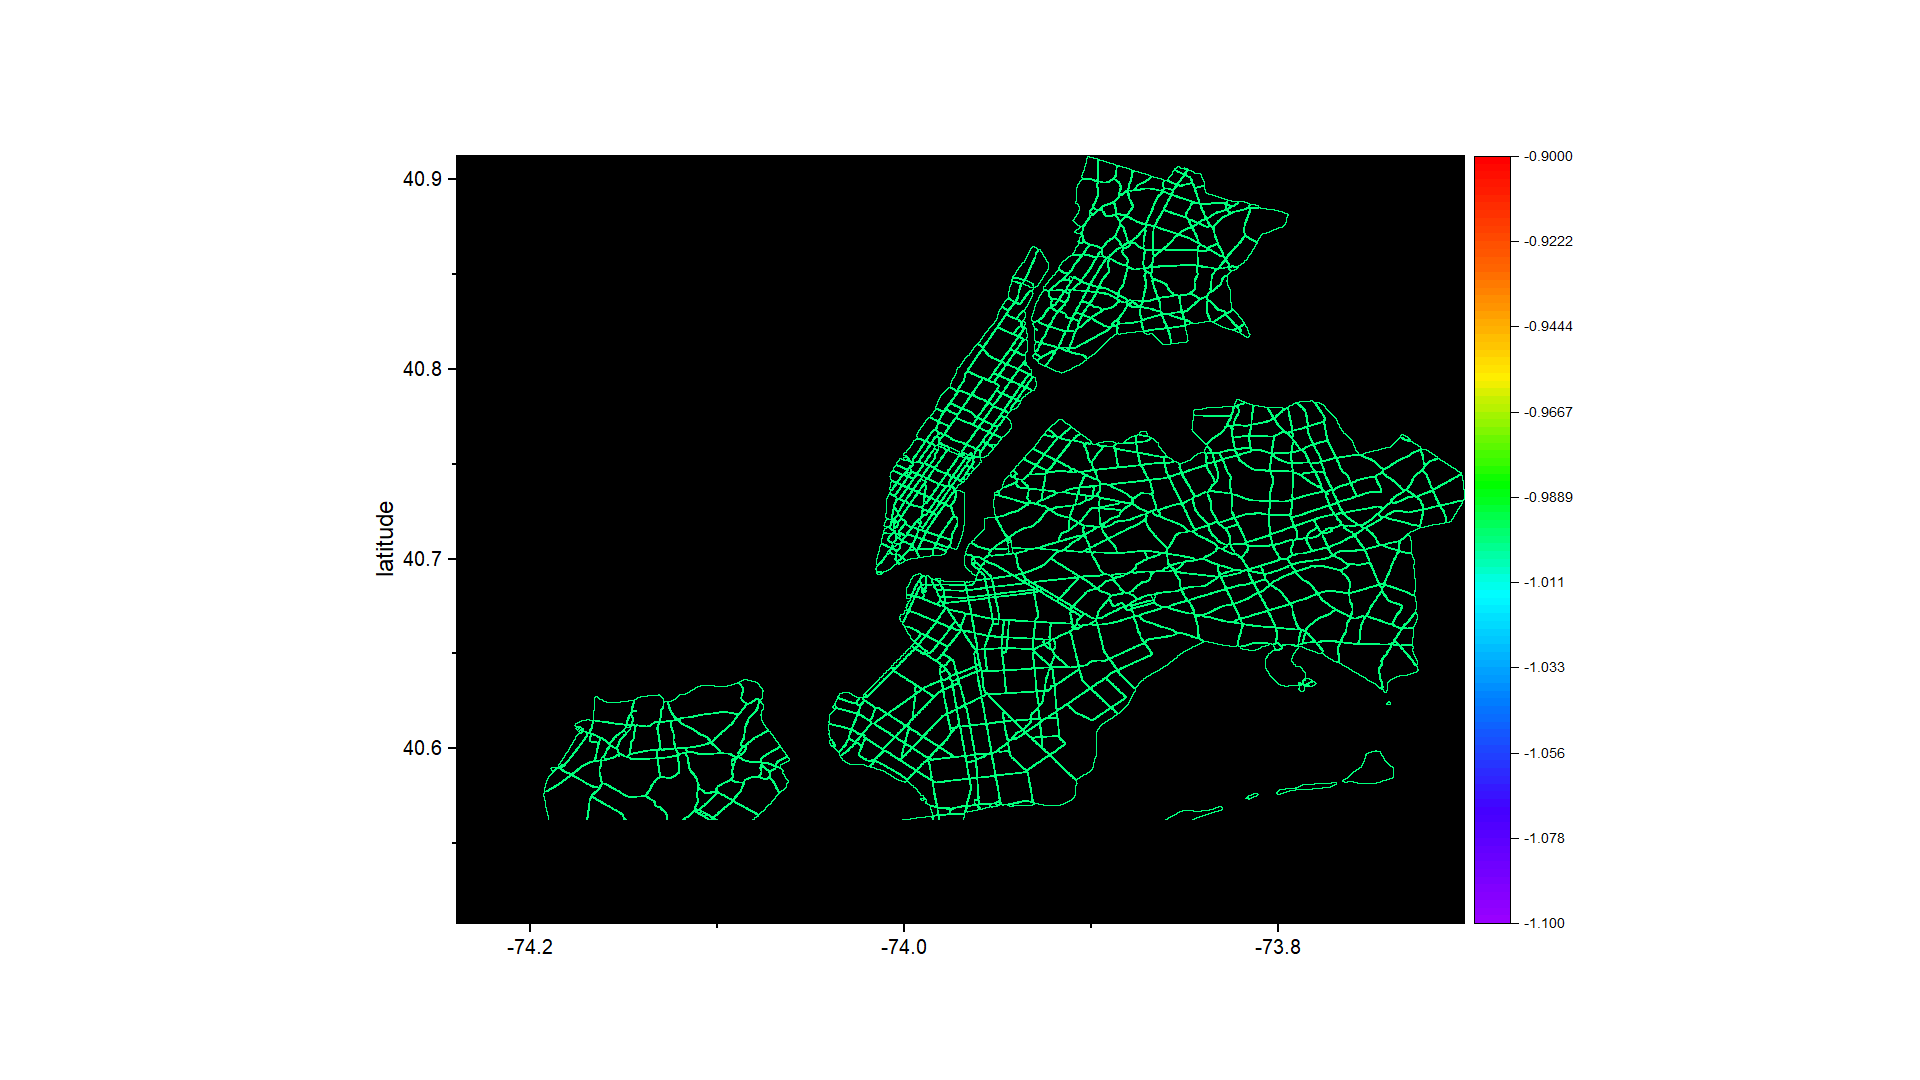
\includegraphics[scale = 0.4]{region.png}
\centering
\caption{区域划分}
\label{figure2}
\end{figure}
\subsubsection*{POI}
第二个数据集是$POI.txt$。数据集包含了不同地区人们的兴趣点的描述,文件总共有862行,每行代表一个区域,一行有$14$个非负数字,代表了$14$种类型各自的数量。
\begin{table}[ht]
\centering 
\caption{POI数据格式}
\begin{tabular}{c|c|c|c|c|c|c}
\toprule 
\tiny{Arts} \& \tiny{Entertainment} &\tiny{Automotive} \& \tiny{Vehicles}&\tiny{Business} \tiny{to} \tiny{Business}&\tiny{Computers} \& \tiny{Technology}&\tiny{Education}&\tiny{Food} \& \tiny{Dining}&\tiny{Government} \& \tiny{Community}\\ \midrule \tiny{Health} 
\& \tiny{Beauty}&\tiny{Home} \& \tiny{Family}&\tiny{Legal} \& \tiny{Finance}&\tiny{Real} \tiny{Estate} \& \tiny{Construction}&\tiny{Shopping}&\tiny{Sports} \& \tiny{Recreation}&\tiny{other}\\
\bottomrule
\end{tabular}
\label{table1}
\end{table}
\subsubsection*{311 complaint}
第三个数据集是$pure\_Four.csv$。311服务请求数据在纽约是开放的,可以自行在网上下载,https://data.cityofnewyork.us/Social-Services/311-Service-Requests-from-2010-to-Present/erm2-nwe9。我从数据开源平台下载了从2010年到现在的所有数据,并从中提取2014和2015年的数据作为实验数据。数据集中的每一行对应着一个投诉,并且对于每一个投诉,都给出了时间地点和投诉类型等信息。将所有的投诉类型划分为四类,进行简单的数量统计,得到如图\ref{311}所示的分布。
\begin{figure}[ht]
\centering
\subfigure[噪声投诉]{
\begin{minipage}[t]{0.4\linewidth}
\centering
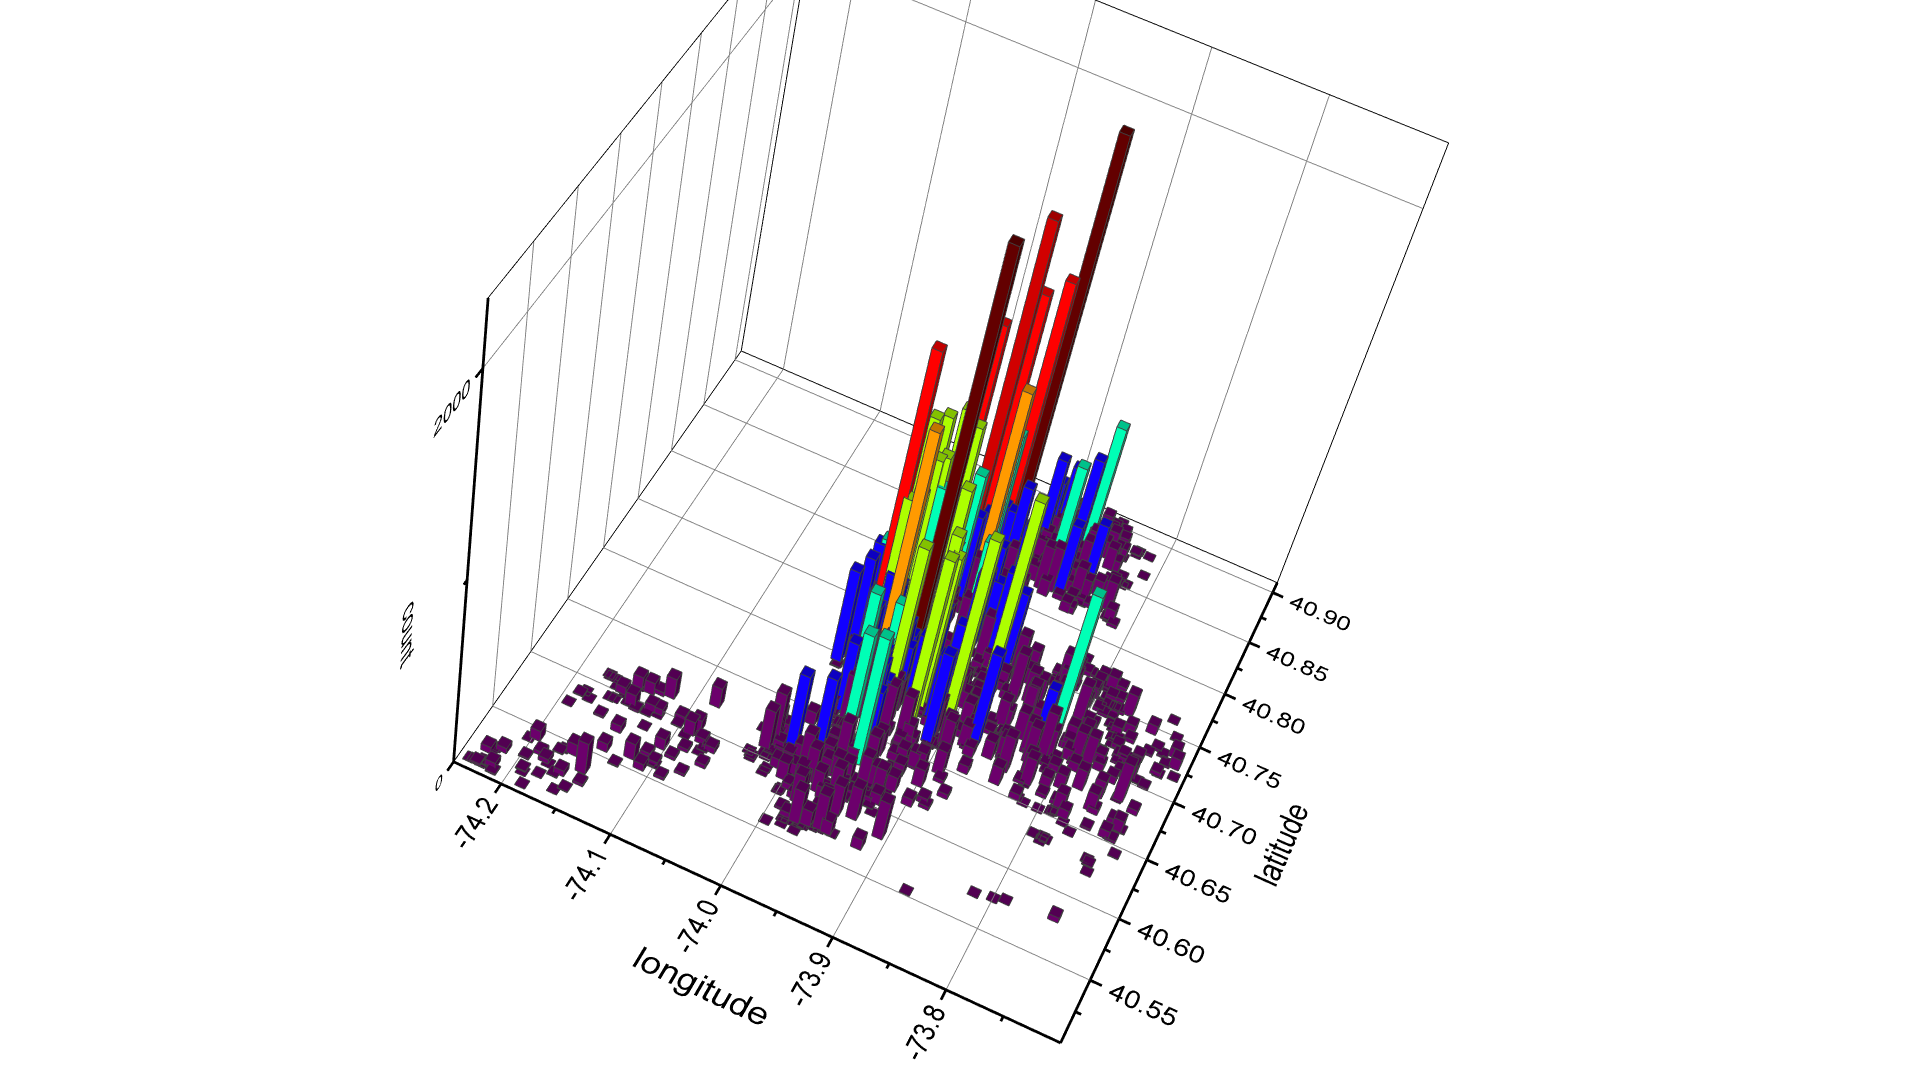
\includegraphics[scale = 0.2]{noise.png}
\end{minipage}
}
\subfigure[非法停车投诉]{
\begin{minipage}[t]{0.4\linewidth}
\centering
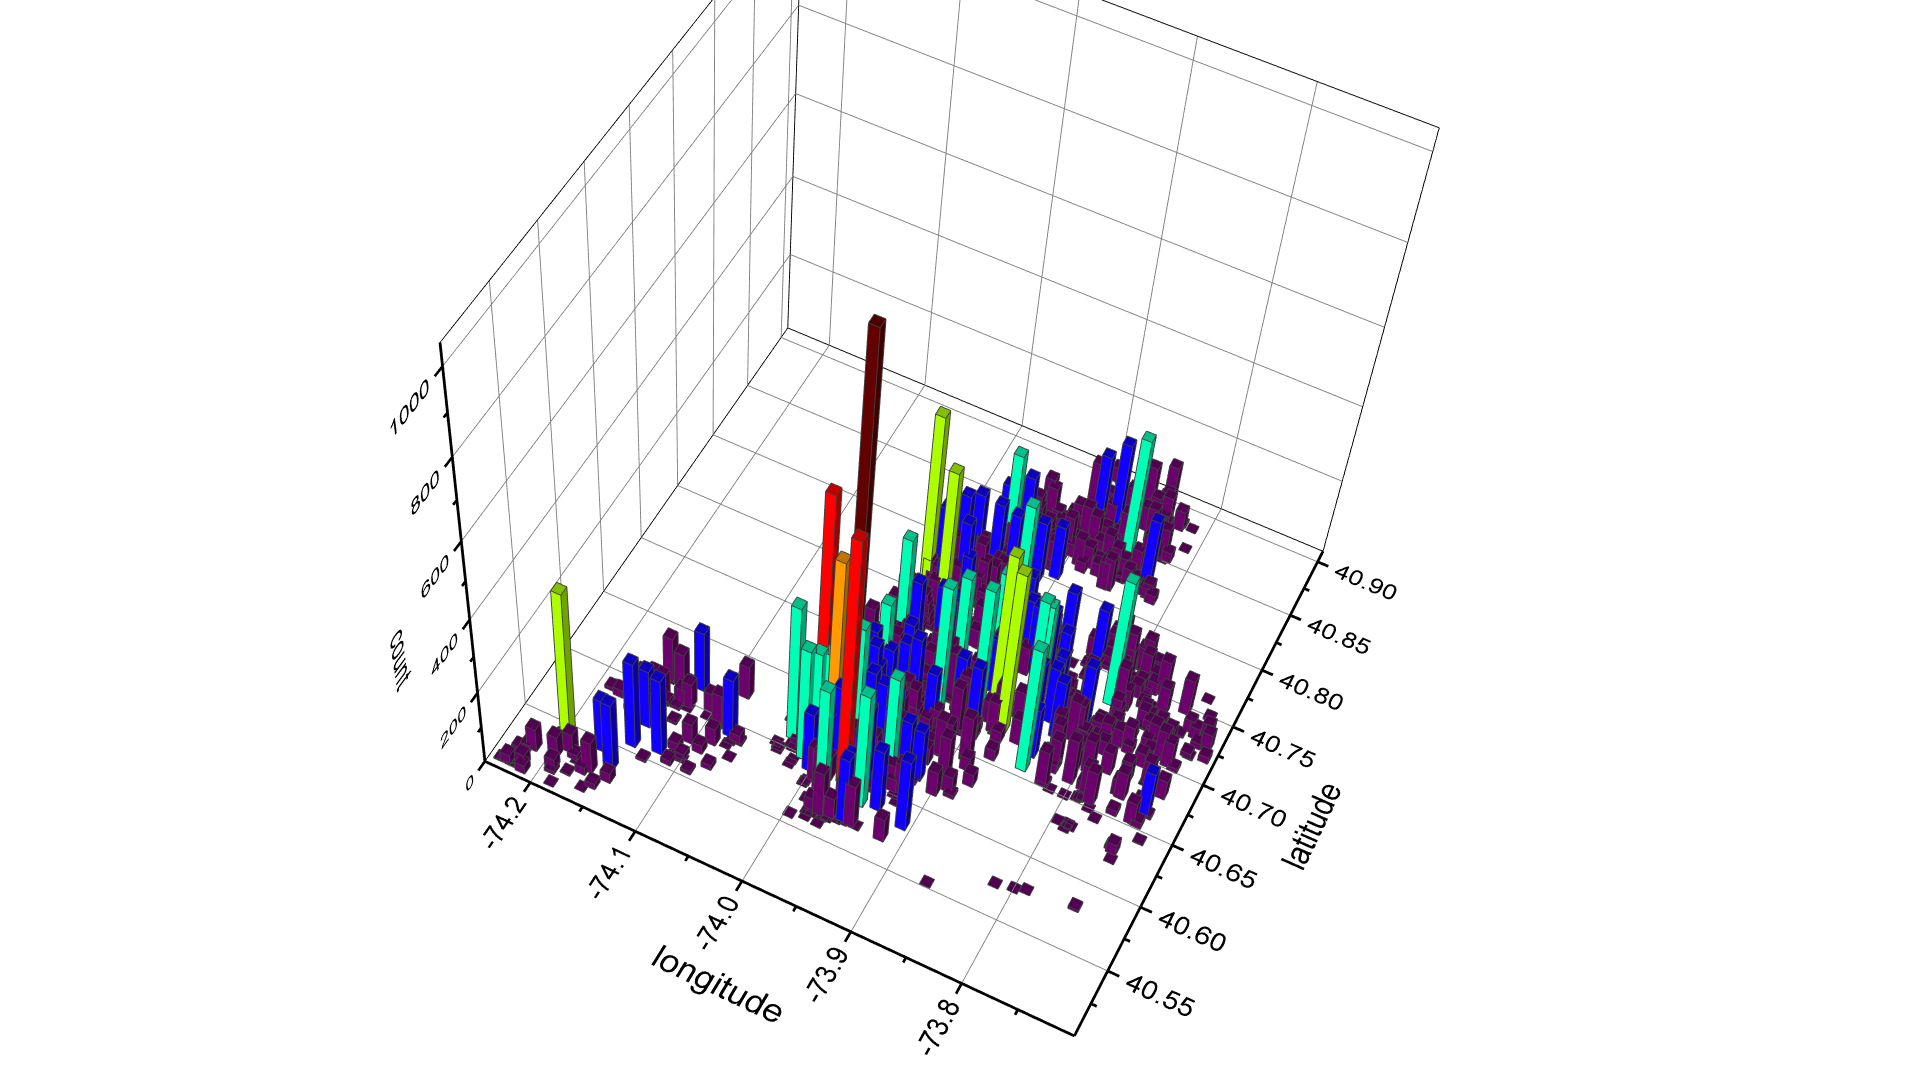
\includegraphics[scale = 0.2]{illegal.png}
\end{minipage}
}
\subfigure[堵塞投诉]{
\begin{minipage}[t]{0.4\linewidth}
\centering
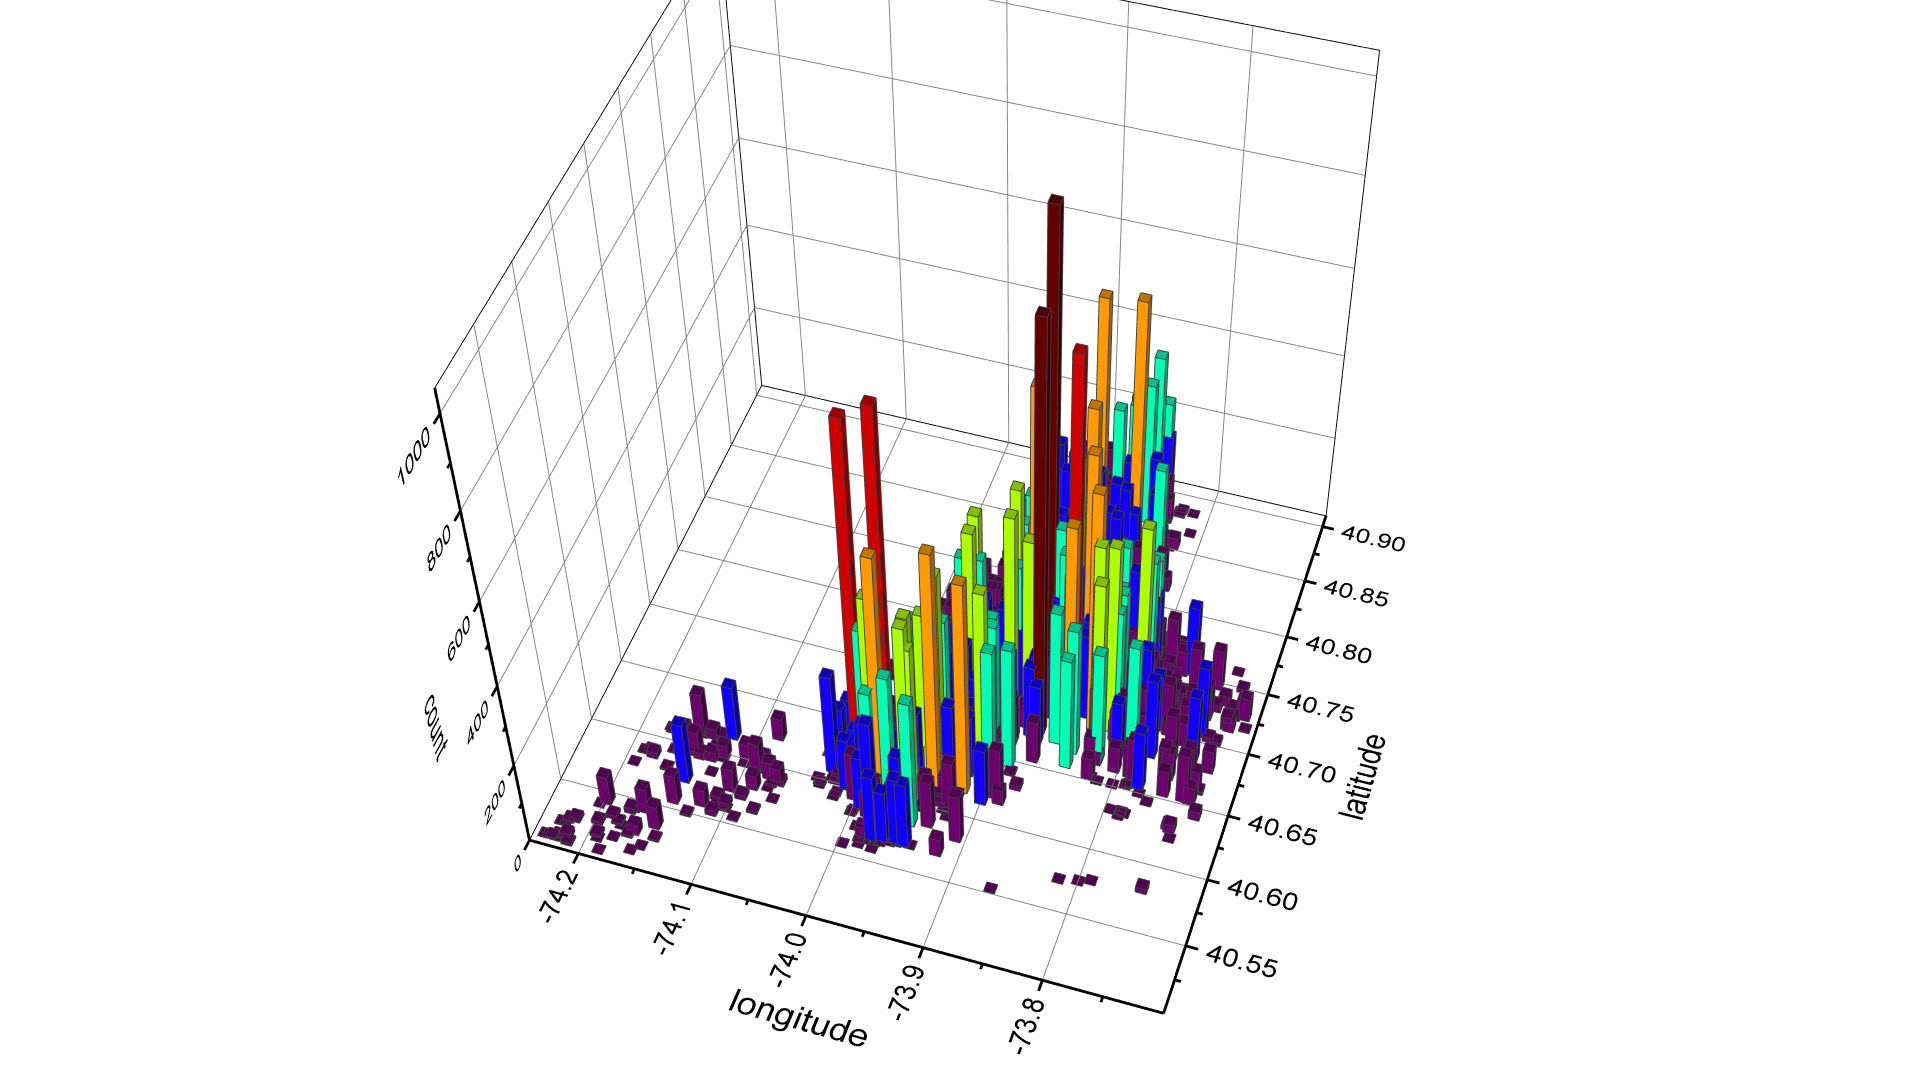
\includegraphics[scale = 0.2]{blocked.png}
\end{minipage}
}
\subfigure[其他类型]{
\begin{minipage}[t]{0.4\linewidth}
\centering
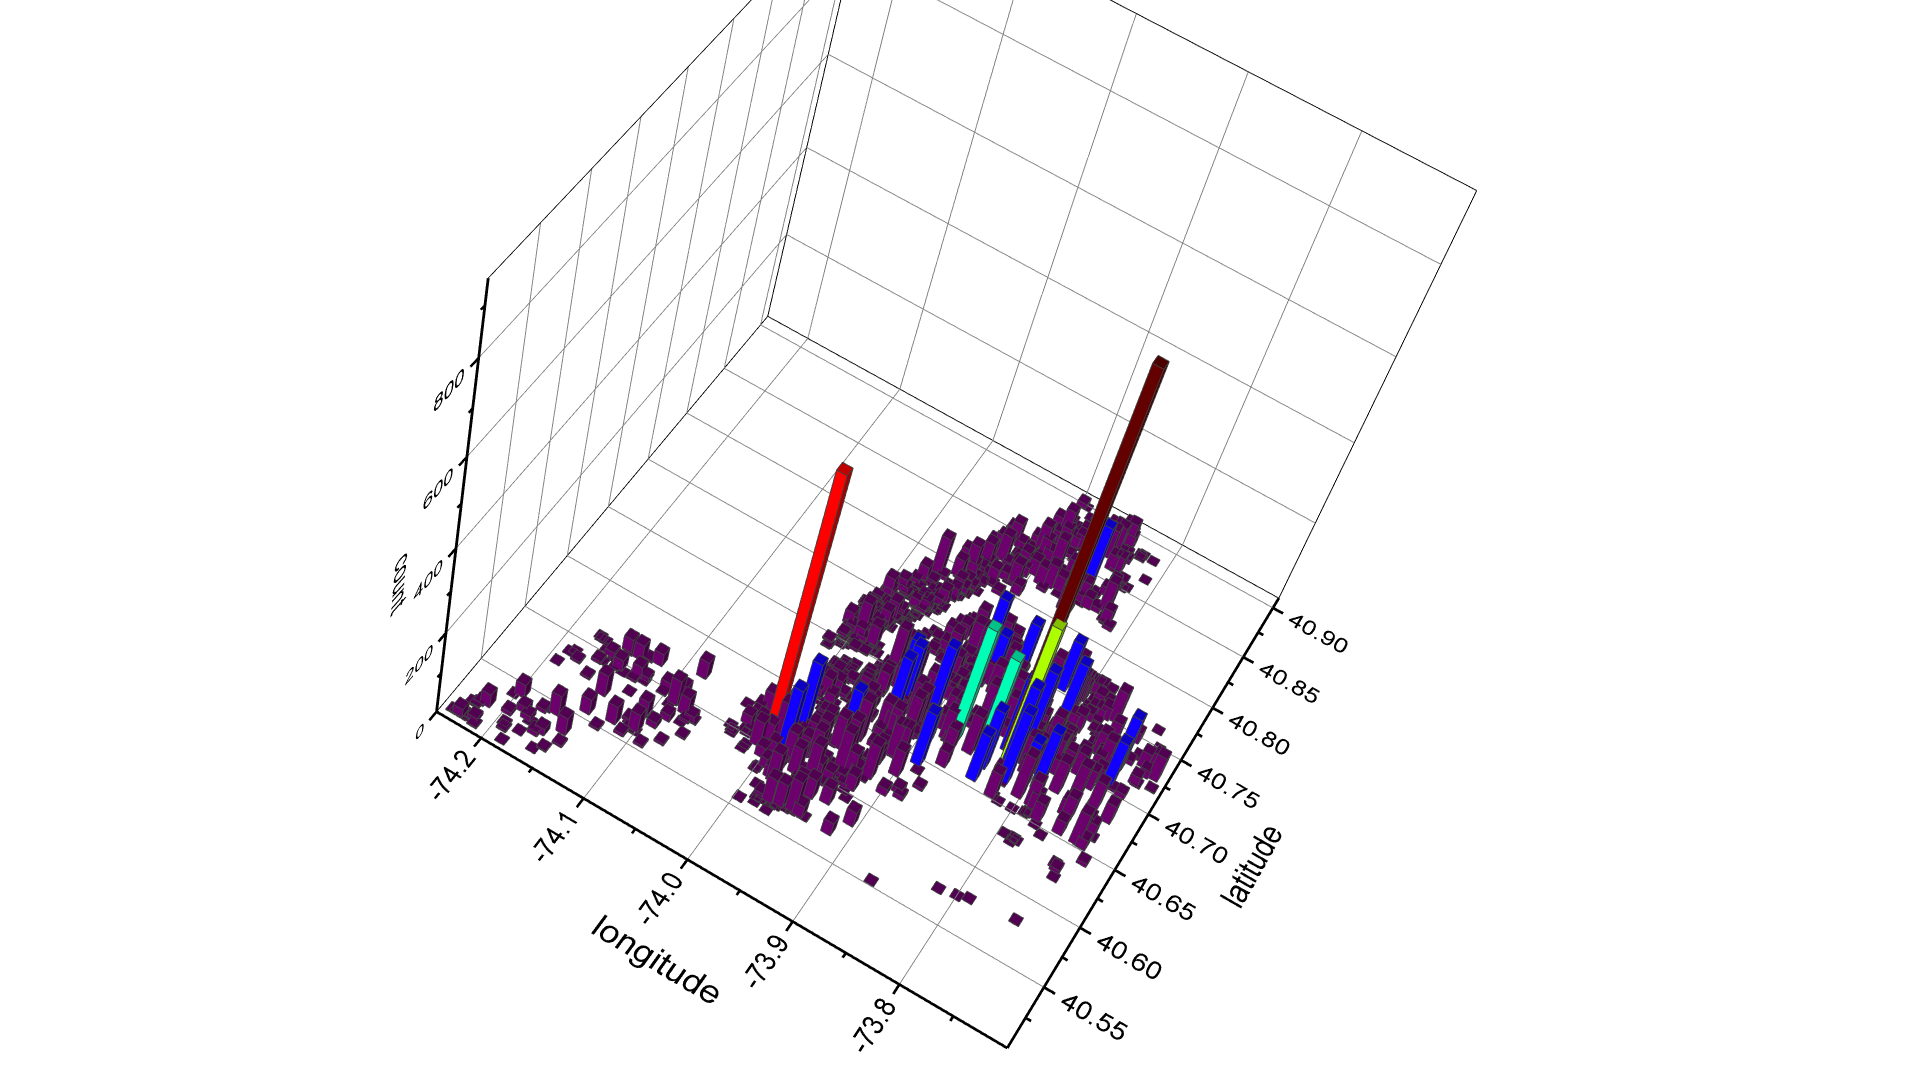
\includegraphics[scale = 0.2]{others.png}
\end{minipage}
}
\centering
\caption{311投诉}
\label{311}
\end{figure}
\subsubsection*{bike}
第四个数据集是$bike.csv$,在官方网站http://www.citibikenyc.com/system-data提供了近年来纽约市单车租界记录全部的数据。我下载了2014和2015两年的数据作为实验数据。如图\ref{bike}\\所示是部分自行车租借记录可视化结果。
\begin{figure}[ht]
%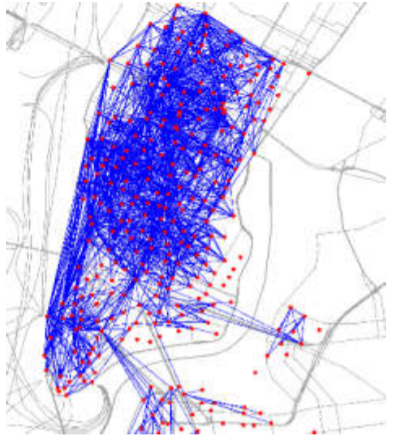
\includegraphics[scale = 0.5]{bike.png}
\centering
\subfigure[自行车租借记录可视化]{
\begin{minipage}[t]{0.45\linewidth}
\centering
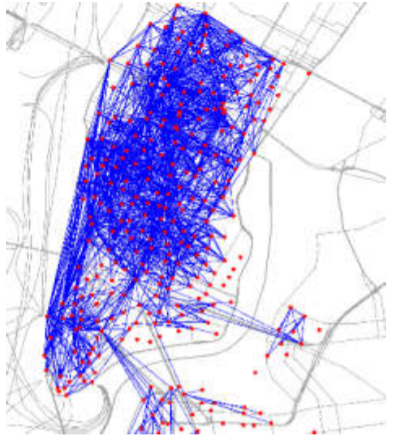
\includegraphics[scale = 0.5]{bike.png}
\label{bike}
\end{minipage}
}
\subfigure[出租车行驶轨迹可视化]{
\begin{minipage}[t]{0.45\linewidth}
\centering
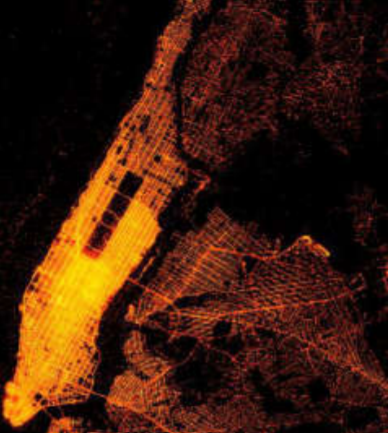
\includegraphics[scale = 0.5]{taxi.png}
\label{bike}
\end{minipage}
}
\caption{自行车和出租车流量可视化}
\end{figure}
\subsubsection*{taxi}
第五个数据集是$taxi.csv$。在官方网站https://data.cityofnewyork.us/browse?q=taxi\%202015 \\ \&sortBy=relevance提供了近年来纽约市单车租界记录全部的数据。我下载了2014和2015两年的数据作为实验数据。每个数据集包括了出发点的经纬度,到达点的经纬度,乘车人数,每单里程等信息。实验重点使用该数据集和下个数据集,关于$bike.csv$,将会在系统的讲解中进一步描述。部分出租车行驶轨迹可视化如图\ref{taxi}所示。
\section{系统}
\subsection{系统框架}
整个系统分为两个模块:训练模块和服务模块。服务模块是最终提供给用户使用的模型,在使用之前需要建立一定的数学模型并进行配置,这部分工作包含在训练模块中。如图\ref{system}所示。
\begin{figure}[ht]
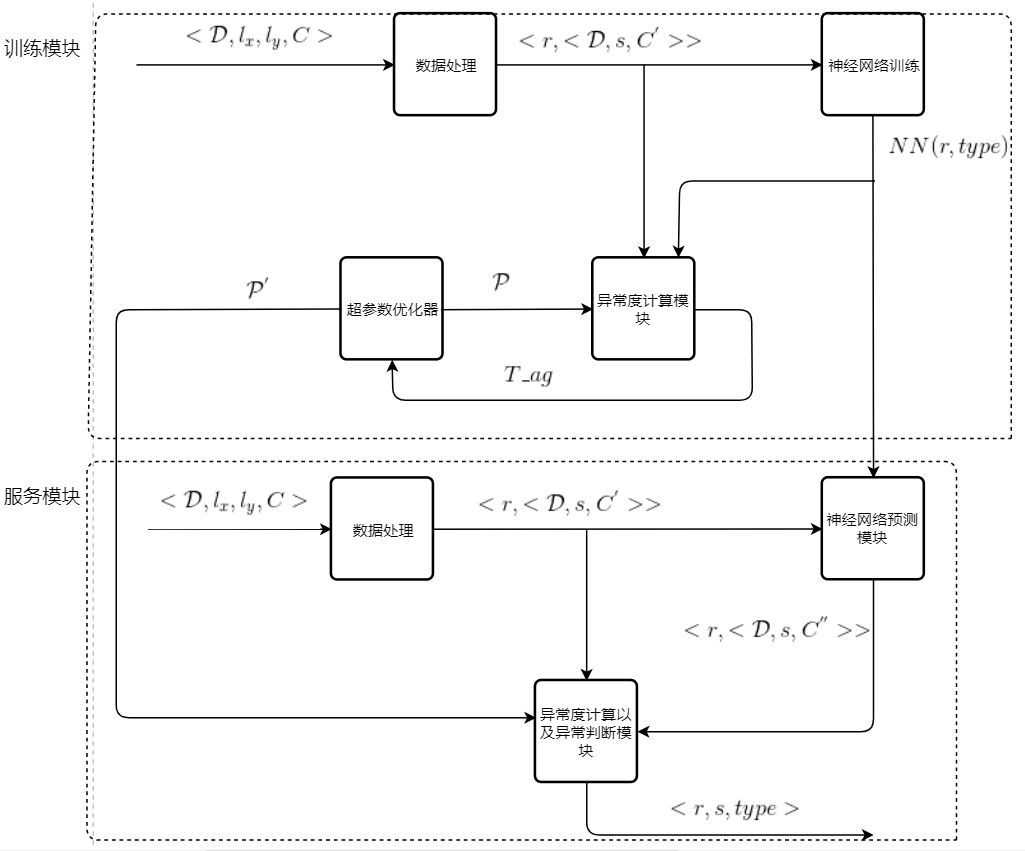
\includegraphics[scale = 0.7]{system.png}
\centering
\caption{系统流程}
\label{system}
\end{figure}
\subsection{模块分析}
\subsubsection*{训练模块}
训练模块分为四个核心部分,他们分别是:数据处理模块、神经网络训练模块、异常度计算模块、超参数优化模块。
\par数据处理模块是一个基于$MapReduce$的并行处理模块,其输入是原始数据$<\mathcal{D},l_x,l_y,C>$,输出是结构化的可处理数据$<r,<\mathcal{D},s,C^{'}>>$。详细实现见技术分析之并行方案。
\par神经网络训练模块用于训练系统中所需的神经网络,训练数据来自数据处理模块给出的数据,输出是训练完成的神经网络。详细定义以及配置见技术分析之拟合分布。
\par异常度计算模块是一个用于计算异常度的数学模型,输入是经过数据处理模块处理过的数据以及神经网络的预测值,输出是每一个地区的整体异常度,它的运行需要配置一定的参数。关于配置信息、异常度计算方法见技术分析之异常度计算模型。
\par超参数优化模块基于贝叶斯优化实现最优超参数的选取,与异常度计算模块一同迭代计算,最终输出模型的最优参数。算法见技术分析之异常度计算模型。
\subsubsection*{服务模块}
服务模块由三部分构成:数据处理模块、神经网络预测模块、异常度计算以及异常判断模块。数据处理和训练模块中的是一样的,神经网络预测模块使用的就是之前已经训练好的神经网络,而异常度计算以及异常判断模块则是在异常度计算模型的基础之上添加了最优参数的配置、异常判断以及异常分类功能,最终输出$<r,s,type>$,$type$中包含着类别信息,这一点将在实验环节进行描述。
\subsection{大作业}
关于大作业中的任务:A.设计大数据分析算法,分析多元数据的分布特征。B.设计异常检测算法,识别数据中的异常事件(地点,起止时间)。C.设计分类算法,对异常事件进行分类。任务A已经在前面的数据模块进行了简单的评述,并在后面的并行方案中进行补充叙述。任务B和C在服务模块的最后一个环节使用,关于其实现原理见于技术分析的后四个章节。
\section{技术分析}
本系统使用了神经网络拟合、贝叶斯优化、并行计算等多种方法来完成完善系统的功能,接下来将会进行一一介绍。
\subsection{并行方案}
设计基于$MapReduce$的方案来加速数据的处理,算法伪代码设计如下:
\begin{breakablealgorithm}
  \caption{基于$MapReduce$的数据处理}
  \centering 
  \begin{algorithmic}[1]
    \Require $<\mathcal{D},l_x,l_y,C>$
    \Ensure $<r,\mathcal{D},s,C^{'}>$
	\Function{REGION\_MAP}{$l_x,l_y$}
	\State $i,j \gets CAL\_INDEX(l_x,l_y)$
	\State $matrix \gets READ\_FILE(region.txt)$
	\State \Return $matrix[i][j]$
	\EndFunction

	\Function{MAP}{$lis<\mathcal{D},r,C>$}
	\State $ans \gets \{\}$
	\For {$entry \in lis$}
		\State $ans[entry[r]].append(<\mathcal{D},C>)$
	\EndFor
	\State \Return $ans<r,lis<\mathcal{D},C>>$
	\EndFunction
	\State
	\Function{REDUCE}{$lis<\mathcal{D},C>$}
	\For {$entry \in lis$}
	\State $entry \gets [entry[\mathcal{D}],CAL_SLOT(entry),C]$
	\EndFor
	\For {$same \mathcal{D} and same s$}
	\State $C \gets C^{'}$
	\EndFor
	\State \Return $lis<<\mathcal{D},s>,C^{'}>$
	\EndFunction
	\State
	\State $\textbf{MAIN}$
	\State $lis \gets $\Call{REGION\_MAP}{$Input[l_x,l_y]$}
	\State $dic \gets $\Call{MAP}{$lis1$}
	\For {$entry \in dic$} 
	\State $entry \gets $\Call{REDUCE}{$entry$}
	\EndFor
	\State \Return $dic$
  \end{algorithmic}
\end{breakablealgorithm}
\par 要将$<\mathcal{D},l_x,l_y,C>$格式的数据转化成$<r,\mathcal{D},s,C^{'}>$格式的数据。输入包含了每一个事件的发生时间,经纬度,事件包含流量;输出包含了事件发生的区域,日期,属于哪一个时间段,该时间段的总流量。在任务执行过程中需要解决三个问题:首先要将经纬度映射到区域的编号上,其次要将不同区域的信息分开,最后是将各个区域内同一个时间段内的流量进行合并。三个问题分别对应了三个$function$。
\par 在实现的时候,有两件事情需要注意:$311 compliant$数据集的处理略有差异,最终$C$以及$C^{'}$分别应该是字符串和字符串列表,每一个字符串对应了一个事件,其内容表示其类型。第二个是这个伪代码是针对每一个数据集的,因此在实际运行的时候需要运行$5$次,基于上述表示,通过并行计算可以获得很好的效率,值得注意的是没有采用现成的并行计算框架,而是自己手写了$MAP,REDUCE$函数,并将程序分配在多个进程中并行执行,起到了相同的效果。
\subsection{拟合分布}
基于数据处理得到的数据,现在可以进行神经网络的训练,考虑到每个地区的差异以及不同数据集的差异,总共需要$862 * 4$个神经网络,$311 complaint$不需要神经网络进行处理,它本来就是稀疏的,并且考虑其含义可以认为只要出现了$complaint$就可以认为出现了一定的异常情况。
\par 值得注意的是此处使用的神经网络结构是简单的,因为拟合的是一个一元分布,输入是时间段编号$s$,输出是预测的该时间段内的流量$predictvalue$。这些数据在上一个部分中已经准备好了。
\par 关于神经网络的参数配置,整个模型是在$keras$上搭建的,使用两个全连接层,第一层输出维度为10,激活函数为$sigmoid$,实用偏置,第二层输出维度为1,没有激活函数,使用偏置,为输出层。训练模型使用的损失函数为$mse$,优化器采用改进的梯度下降法$RMS$,并且采用回调函数是学习率随时间递减,数据集使用100次,即$epoch = 100$。训练结束之后将模型保存在相应的$.h5$文件中,在随后进行调用时,直接从文件中导入模型并进行预测。关于文件名请见目录结构,如图\ref{file}所示。
\begin{figure}[ht]
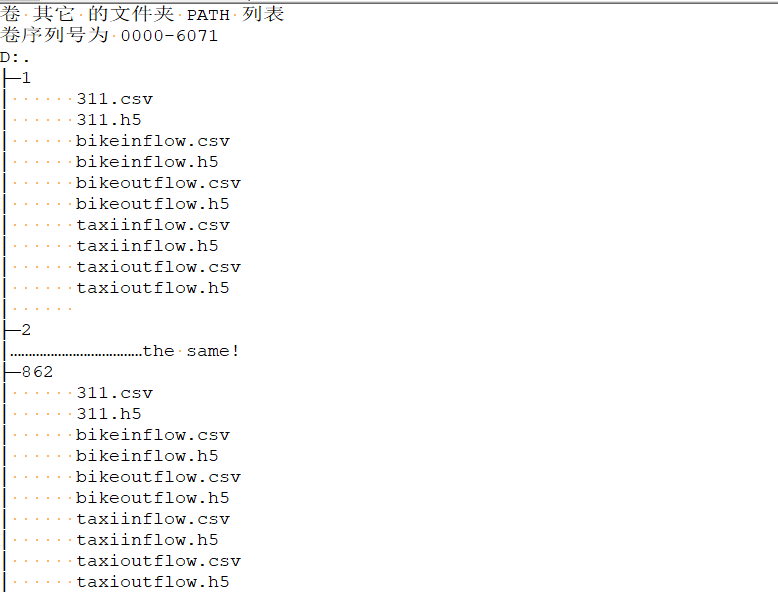
\includegraphics[scale = 0.5]{structure.png}
\centering
\caption{文件结构目录}
\label{file}
\end{figure}
\subsection{异常度计算模型}
异常度计算分为三个阶段,先计算单个地区单个数据集的异常度,其次计算跨数据集影响的异常度,最后计算跨地区影响的异常度,计算方法见算法2。
\begin{breakablealgorithm} 
  \caption{计算异常度}  
  \label{alg:Framwork}  
  \begin{algorithmic}[1]
    \Require 没有输入,当前时段数据更新
    \Ensure 计算整体异常度
	\Function{SINGLE\_DATASET}{$t$}
	\State $CONTRIBUTION \gets [0.5,0.25,0.125,... ...]$
	\State $ag_t \gets \sum_{i \in [0,47]}{\frac{|realvalue_{i} - predictvalue_{i}|}{realvalue_{i}}} * CONTRIBUTION[i]$
	\State \Return $ag_t$
	\EndFunction
	\State
	\Function{ACROSS\_DATASET}{$ag_1,ag_2,ag_3,ag_4,sign$}
	\State $w_1,w_2,w_3,w_4,ag311\gets values fome file$
	\State $w_5 \gets sign,ag_5 \gets ag311$
	\State $\varphi_i \gets w_i * ag_i$
	\State $ag^{'} = \sqrt{\frac{\sum_{i \in m}{\varphi ^ {2}}}{m}}$
	\State \Return $ag_{'}$
	\EndFunction
	\State
	\Function{ACROSS\_REGION}{$ags$}
	\State $\epsilon \gets 0.5$
	\For {$r \in ags.keyset$}
	\State $S \gets ADJACENT(r)$
	\State $ags[r] \gets \epsilon * ags[r] + \sum_{i \in S}{\frac{1 - \epsilon}{|S|}ags[i]}$
	\State \Return $ags$
	\EndFor
	\EndFunction
	\State $\textbf{MAIN}$
	\State $S \gets all datasets$
	\State $R \gets all regions$
	\State $ans \gets \{\}$
	\For {$r \in R$}
		\State $tmpag \gets []$
		\For {$s \in S$}
		\State $tmpag.apend(SINGLE\_DATASET(s))$
		\EndFor
		\State $ans[r] \gets ACROSS\_DATASET(tmpag[0],tmpag[1],tmpag[2],tmpag[3])$
	\EndFor
	\State $ans \gets ACROSS\_REGION(ans)$
	\State \Return $ans$
	\State
  \end{algorithmic}  
\end{breakablealgorithm}
\par 在计算单个数据集的异常度时使用的是之前24小时的所有相关数据,每一个时间段对应一个,也就是48个数据,但是数据的权重是不一样的,所以定义$CONTRIBUTION$进行加权,距离当前时间结点最近的权重最高,为0.5,之后依次按照$1/2$递减,当权重小于一定值时将所有的值设置为$\epsilon$,即一个很小的数。最终算法返回的是一个地区的某个数据集在特定时段下的异常度计算结果。
\par 在计算跨数据集的异常度时,先不考虑地区的因素,总共有$5$个数据集需要考虑,其中311数据集不需要进行单个异常度的估计,而是用一个指示变量$sign$代替,如果变量值为1,就表示$311$数据集产生异常,否则没有产生异常,置0。因为每一个数据集的贡献可能不同,所以之后进行加权得到$\varphi_i$,最后对得到的$\varphi_i$数组求方差得到跨数据集的异常度。需要注意的是在这里有三个参数需要配置,关于配置方法在贝叶斯优化部分进行讲述。
\par 在完成了前面两步的计算之后,开始计算跨地区的异常度,对于一个确定的地区$r$,我们只考虑其本身的异常度以及其相邻区域的异常度,并给他们附上不同的权重,其中本身的权重占$0.5$,其余的权重相邻的区域平均分配。
\subsection{贝叶斯优化}
在上一个部分的讲解中已经指出了一部分参数,除了$4$个权重和$311$异常度之外,还有$48$个超参数,在我的模型中认为,不同时段的流量是不同的,而且投诉一般发生固定的几个时段,所以有必要对每个时段分别设置阈值。综上所述,总共有$53$个超参数需要进行配置。
\par 于是系统到这里就变成了一个调参数问题,需要定义目标函数,优化方法,训练数据,并确定搜索空间。训练数据参考论文中引述的异常事件,不使用这些数据,而是参考其数据分布特征在历史数据中寻找异常数据,因为这些数据在实验中还要使用,将训练集和验证集分开是必要的。经过比较确定搜索算法为$TPE$,搜索空间指定为所有在超参数在$[0,1]$之间服从均匀分布。实现使用$python$的开源库$hyperopt$,定义目标函数为$fmin(errorrate, space, algo=algo)$,后两个变量已经声明过了,关于目标函数$errorrate$见伪代码3。
\begin{breakablealgorithm}
  \caption{errorrate}
  \begin{algorithmic}[1]
    \Require $w0,w1,w2,w3,w4,ag311,$\\
              $threshold0,threshold1,threshold2,threshold3,threshold4,threshold5,$\\
              $threshold6,threshold7,threshold8,threshold9,threshold10,threshold11,$\\
              $threshold12,threshold13,threshold14,threshold15,threshold16,threshold17,$\\
              $threshold18,threshold19,threshold20,threshold21,threshold22,threshold23,$\\
              $threshold24,threshold25,threshold26,threshold27,threshold28,threshold29,$\\
              $threshold30,threshold31,threshold32,threshold33,threshold34,threshold35,$\\
              $threshold36,threshold37,threshold38,threshold39,threshold40,threshold41,$\\
              $threshold42,threshold43,threshold44,threshold45,threshold46,threshold47$
    \Ensure $rate$
	\State $Data \gets\ source\ from\ file$
	\State $num \gets 0$
	\For {$entry \in Data$}
	\State $sign \gets 0$
	\State $T_{ag} \gets AG(entry)$
	\State $threshold \gets THRESHOLD(entry)$
	\If {$T_{ag} > threshold$}
	\State $sign \gets 1$
	\EndIf
	\If {$sign \neq entry.label$}
	\State $num \gets num + 1$
	\EndIf
	\EndFor
	\State \Return $num / len(Data)$
  \end{algorithmic}  
\end{breakablealgorithm}
\par 对数据集中每一条数据都进行预测,对错误的预测进行计数,最后除以总的个数,结果就是错误率,目标函数为最小化函数,也就是使这个值尽量的小从而实现整个参数优化的过程。
\subsection{分类方案}
在整个数据处理结束之后,还需要对异常结果进行分类。考虑到实际的情况,有意义的分类是指出当前异常的规模有多大,从而对异常有一个整体的把握;指出异常带有什么样的标签,从而能够制定针对异常的解决方案。于是提出如下分类方法:经计算得到当前时间段所有的异常区域之后,得到的结构化数据为$<r_1,r_2,...>$。首先将相邻的区域进行合并,这是一个求解连通分量个数的问题,也是一个求解最大独立子集合个数的问题,在这里我的处理方法为第二种。维护一个并查集,检查每一个异常的地区,如果这个地区的相邻地区发生异常,就将这两个地区合并,映射到数据结构中就是进行并查集的$find$操作。最终并查集中留下了所有独立的区域集合$<r_1^{'},r_2^{'},...>$,$r_i^{'} = \{r_{t_1},r_{t_2},r_{t_3},...\}$。按照区域的大小对异常进行分类,并在$report.csv$中输出结果时,将每一个区域集合的$label$都进行输出,作为此次异常该区域集合的异常标签。总之,分类的结果就是$<level,labels>$,其中$level$是异常等级,$labels$是异常标签。
\section{实验}
\subsection{实验设计}
在进行实验之前已经使用2015一年的数据对系统中用于预测的神经网络进行了训练,并且对系统中的超参数进行了最优的标定,在实验中使用2014年的数据进行异常检测。
\par 为了直接利用论文中的实验结果(对$2014-10-31$到$2014-11-27$的数据进行了异常检测)进行对比,将该时间段的数据运行在本系统上,作为实验。
\par 论文里实验数据中的异常事件是从$nycinsiderguide.com$网站获取的,为了方便实验结果展示,在此对异常事件进行编号,如图\ref{anomaly}所示。
\begin{figure}[ht]
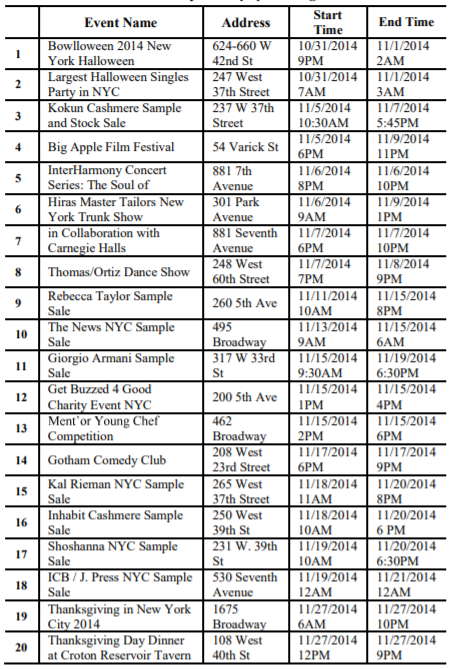
\includegraphics[scale = 1]{event.png}
\centering
\caption{异常事件示例}
\label{anomaly}
\end{figure}
\par系统运行结束之后输出检测到的异常事件所在区域和相应的时间区间。首先检查时间段和图\ref{anomaly}给出的时间段是否吻合,然后再在地图($http://api.map.baidu.com/lbsapi/getpoint$)上搜索对应区域的中心点的经纬度坐标,找到相关区间并检查是否包含发生异常事件的街道地址,如果以上两点都能满足,则认为一条异常预测成功。
\par 值得注意的一点是,本系统进行异常检测依赖于当前时间点以及此前24小时的数据分布,所以本系统运行的起点是$2014-10-30$的数据,但是异常检测的起点是$2014-10-31$。
\subsection{对比实验}
在对比实验中设置七个对照组,他们分别是$DB-S-Taxi-S$,$DB-S-Taxi-B$,$DB-S-Bike-S$,$DB-S-Bike-B$,$DB-M-One$,$DB-M-All$,$ST-LRT$。其中前四个实验是使用单一原始数据集的,后面三个是跨数据集的检测,对照组数据配置信息如图所示。
\begin{figure}[ht]
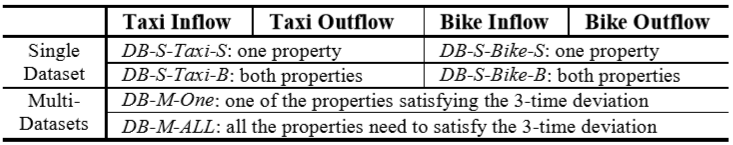
\includegraphics[scale = 0.6]{experiment.png}
\centering
\caption{对照组数据配置信息}
\end{figure}
\par 而本系统在运行时基于三个源数据集$bike$,$taxi$,$311$对异常进行检测。





\subsection{实验结果}
将算法检测出的异常事件的编号和算法对应,制作成表格,如表\ref{ending}所示。

\begin{table}[ht]
\centering
\caption{检测到的异常事件对比}
\label{ending}
\begin{tabular}{l|r}
\toprule 
\normalsize{\textbf{方法}} & \normalsize{\textbf{检测到的异常事件编号}}\\
\midrule
\normalsize{DB-S-Taxi-S} & \normalsize{$1,9,19,20$}\\
\normalsize{DB-S-Bike-B} & \normalsize{$9,19,20$}\\
\normalsize{DB-S-Taxi-B} & \normalsize{$4,19$}\\
\normalsize{DB-S-Bike-B} & \normalsize{$None$}\\
\normalsize{DB-M-One} & \normalsize{$1,4,9,19,20$}\\
\normalsize{DB-M-All} & \normalsize{$None$}\\
\normalsize{ST-LRT} & \normalsize{$1,3,9,10,11,13,15,16,20$}\\
\normalsize{本系统} & \normalsize{$1,3,4,9,10,11,14,15,16,19,20$}\\
\bottomrule
\end{tabular}
\label{table1}
\end{table}
\par从数量上来看,本系统检测到了更多的异常,也基本覆盖了前面七种方法检测出的异常。结果输出保存在$report.csv$文件中,文件中除了检测到的异常事件$<region,time>$,还对异常区域进行了聚合作为本次大作业任务$C$的结果,异常事件跨越的区域越多,相应的规模等级也越高。
\subsection{实验受参数的影响}
在贝叶斯优化部分已经对参数进行了详细的分析以及标定,在分析问题时将城市的异常检测抽象成了一个超参数优化问题,这些所有的超参数基于历史数据进行训练,并使用贝叶斯模型进行超参数的优化。所以本系统对参数的依赖较大,但是拥有大量的历史数据使得找到最优化的参数成为可能。
\par 除了能够对参数进行合理标定之外,系统的多个参数也为系统增加了一定的灵活性,每经过一段时间,根据这一段时间产生的新的数据进行批处理训练更新参数,从时间维度上使得模型具有更好的适用性。
\section{相关工作}
近十年来,异常检测已经被人们进行了广泛地研究\cite{Chandola2009Anomaly}。在这篇文章里,我只是从时空数据集中进行了相关研究,比如检测异常轨迹\cite{LeeTrajectory}、基于轨迹识别交通异常、发现城市规划中的问题等等\cite{Wei2011Discovering}。因为一个数据集从某个方面真实地描述了一个事件,所以很多潜在的问题可以被挖掘出来。但是也正是因为单个数据集仅仅从一个方面描述了数据集,有很多异常是无法通过单一的数据集发现的。
\par 近年来,一些研究人员开始将多个数据集结合起来来检测异常。在2015年,上海交通大学相关研究人员发表的一篇论文中\cite{DalzielDetecting},首次考虑了跨越多个地区的影响,进行一个整体的检测,发现可以得到更好的效果。
\par 从上交研究人员的工作出发,除了空间和多元数据集,我将时间维度纳入考虑,并且分析了拟合流量的更好的方法,成功地将问题抽象成一个基于历史数据的、自适应的超参数优化模型,并且为其设计大数据实时计算方法,从而实现从批处理到实时处理的转变。
\section{结论}
在综合了前人工作的基础之上,从大量的历史数据出发,使用神经网络拟合分布,将时间影响因素纳入考量,为异常检测建立数学模型,将整个问题转化成为一个超参数的优化问题。在完成实验任务的同时,系统取得了不错的结果。为了能使程序运行在分布式系统上,给系统设计了$MapReduce$的接口实现以及数据细节处理,能够较快速的交付对异常事件的预测。撰写专利申请书一份,见附录。
\bibliographystyle{IEEEtran}
\bibliography{ref}
\newpage
\begin{appendix}
\section*{附录-专利申请书}
\subsection*{一、本发明的名称}
面向多元数据的城市整体异常检测实时计算系统
\subsection*{二、本发明的背景}
传感技术和大规模计算基础设施的进步产生了各种各样的城市数据,例如交通流、人的流动性和社会媒体。这些数据集通常与时空信息相关。当它们一起存放时就可以代表城市的动态和节奏。按照前人的工作,整体异常分为两个类别,一个是考虑在一段时间内跨越多个数据集产生异常,针对这一种检测,一般是发现潜在的尚未发展起来的危害,另一个是在一段时间内跨越多个地区产生异常,但是仅仅通过一个地区的数据却没有办法检测出来。如图\ref{m-dataset}所示,三个图片分别展示了不同的数据集对异常的表现,并且在每一张图片中都有异常的中央区域与周边区域的交互信息。
\par为了进行城市整体异常的检测,有三个具有挑战性的问题需要解决:第一个是数据集信息的整合,比如数据集中哪些信息是有用的,有些数据集稀疏,有些数据集稠密,如何对不同格式的数据集进行基于$MapReduce$的统一的处理;第二个是数据集分布的拟合以及异常度的确定,在进行拟合时,数据集可能服从多种分布,也有可能在不同的时段服从不同的分布,如何进行统一的处理,并在拟合分布的基础上进行异常度的计算;第三个是信息的合并,这一点主要是跨数据集和跨地区的信息合并。
\subsection*{三、现有的技术缺陷}
一个比较好的系统就是2015年上海交通大学发表的论文中提出的模型。整体的思路即假设$311 complait$数据集中的数据服从高斯分布,车流数据服从的是泊松分布。使用$\kappa ^ 2$检验检测异常,再采用加权平方和的方法实现跨数据集跨地区的异常检测。
\par论文中一个不合理的假设就是数据集服从某个分布,确实数据集在某个时段内表现服从高斯分布,但是也不是较为标准的分布模型,从一整天来看,与高斯分布模相去甚远,如果按照高斯分布进行检验,计算出的异常度就会很大。换言之,之前的方法解决了整体异常的检测问题,但是检测的太过于宽泛,从而带来不必要的麻烦。其次,论文中并没有考量跨时间的影响因素,这使得有一些异常无法被判断出来。
\subsection*{四、本发明的目的}
针对现有技术的缺陷,我提出了相应的解决方案,从而对整体异常检测系统做进一步的完善。并且为使本系统能够进行即时处理并实时汇报,面向大数据实时处理框架给出$MapRe$-$duce$的接口实现。
\par总之本系统的目的有四。第一,对于提取数据集的分布特征,使用神经网络基于大量历史数据进行拟合。从而替代原有的有关分布的假设,并且充分利用历史数据。第二,在$NN$拟合的基础之上进行包含时间因素的异常度计算,进行跨数据集、跨地区、跨时间区间的异常度计算,设计异常判断算法。第三,设计分类算法,对异常级别分类。第四,设计实现$MapRe$-$duce$接口程序,并且使系统能在大数据实时处理框架上运行。
\subsection*{五、本发明的方案}
\subsubsection*{系统框架}
整个系统分为两个模块:训练模块和服务模块。服务模块是最终提供给用户使用的模型,在使用之前需要建立一定的数学模型并进行配置,这部分工作包含在训练模块中。如图\ref{f-system}所示。
\subsubsection*{训练模块}
训练模块分为四个核心部分,他们分别是:数据处理模块、神经网络训练模块、异常度计算模块、超参数优化模块。
\par数据处理模块是一个基于$MapReduce$的并行处理模块,其输入是原始数据$<\mathcal{D},l_x,l_y,C>$,输出是结构化的可处理数据$<r,<\mathcal{D},s,C^{'}>>$。详细实现见技术分析之并行方案。
\par神经网络训练模块用于训练系统中所需的神经网络,训练数据来自数据处理模块给出的数据,输出是训练完成的神经网络。详细定义以及配置见技术分析之拟合分布。
\par异常度计算模块是一个用于计算异常度的数学模型,输入是经过数据处理模块处理过的数据以及神经网络的预测值,输出是每一个地区的整体异常度,它的运行需要配置一定的参数。关于配置信息、异常度计算方法见技术分析之异常度计算模型。
\par超参数优化模块基于贝叶斯优化实现最优超参数的选取,与异常度计算模块一同迭代计算,最终输出模型的最优参数。算法见技术分析之异常度计算模型。
\subsubsection*{服务模块}
服务模块由三部分构成:数据处理模块、神经网络预测模块、异常度计算以及异常判断模块。数据处理和训练模块中的是一样的,神经网络预测模块使用的就是之前已经训练好的神经网络,而异常度计算以及异常判断模块则是在异常度计算模型的基础之上添加了最优参数的配置、异常判断以及异常分类功能,最终输出$<r,s,type>$,$type$中包含着类别信息,这一点将在实验环节进行描述。
\subsection*{六、本发明的创新点}
本系统的创新点有五个。
\par第一,使用神经网络拟合历史数据,而不是直接假设数据是服从高斯分布。神经网络具有拟合一定场景下的数据分布规律的先天优越性,即使是某一天的数据恰好服从高斯分布,神经网络也能很好的拟合出来。并且训练基于大量的历史数据,是一种对数据的挖掘和价值提升。也正是由于对数据的依赖性,使得模型能够根据数据的不断更新而自动更新,使得模型具有更好的时效性,能够很好的反应当前的真实状况。
\par第二,设计异常度计算算法,在$NN$拟合的基础之上进行异常度计算,首次将时间因素考虑在内。扩大了信息维度,可以是模型具有更好的性能。值得注意的是,由于这一步的存在,系统引入了很多参数,但是由于大量历史数据以及超参数优化算法的存在,这将不再是一个问题。
\par第三,将问题求解转化成了超参数的优化问题。给出了优化的目标函数,需要优化的参数,训练的数据来源,将问题从一个陌生的领域转换到一个比较热门的领域,增加了研究的方法以及研究的可参考性。
\par第四,设计基于并查集的分类算法,对异常级别分类。从划分区域开始,直到使用并查集分类结束,完成了从一整块区域到画出指定的异常区域的任务。在计算的过程中每个区域扫一遍即可完成任务,具有很高的时间效率。
\par第五,设计实现$MapReduce$接口程序,并且使系统能在大数据实时处理框架上运行。数据的处理是重复的,并且数据之间没有依赖,这正是并行处理的最佳数据对象。使用$MapRe$-$duce$可以极大地提高运行效率,从而使系统转化成为一个实时应用系统成为可能。
\subsection*{七、本发明的效果}
与之前的方法相比,本系统具有很好的效果,具体体现为以下几点:
\subsubsection*{更高的精度}
相比于领域内的其他工作,本系统考虑了更多的影响因素,只要训练时间足够,就能对历史数据中的额信息进行充分的提取,从而更好地反应现实世界对应的数据世界。
\subsubsection*{更高的效率}
为了对效率进行保证,本系统做了两部分的工作,一个是基于$MapReduce$的原理缩短数据预处理时间,另一个是基于数据结构的优化对数据的最终处理进行了加速。
\subsubsection*{时效性}
数据是不断产生的,系统运行的最优参数很可能随着时间变化,而本系统是可训练的,在使用时可指定一个时间长度,定期根据最新历史数据进行参数优化,从而适应最新的数据变化,所以具有较好时效性。
\subsection*{八、附图}
\begin{figure}[ht]
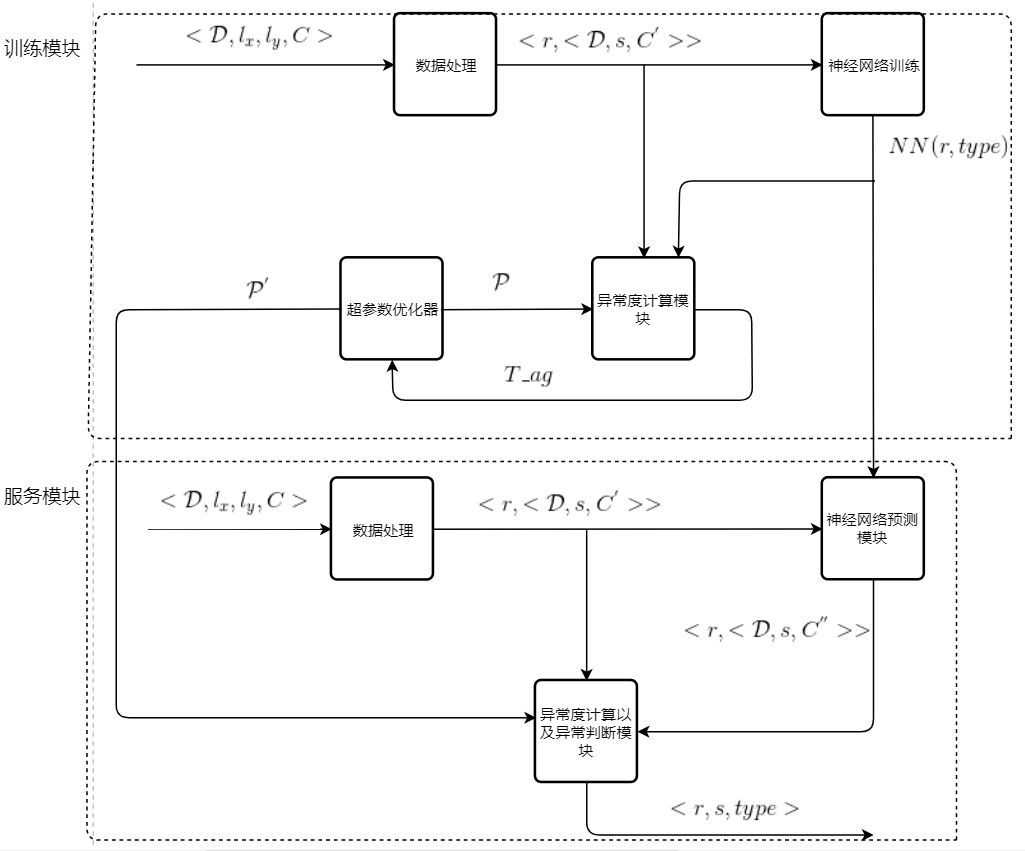
\includegraphics[scale = 0.7]{system.png}
\centering
\caption{系统流程}
\label{f-system}
\end{figure}
\end{appendix}


\begin{figure}[ht]
\centering
\subfigure[噪声投诉]{
\begin{minipage}[t]{0.4\linewidth}
\centering
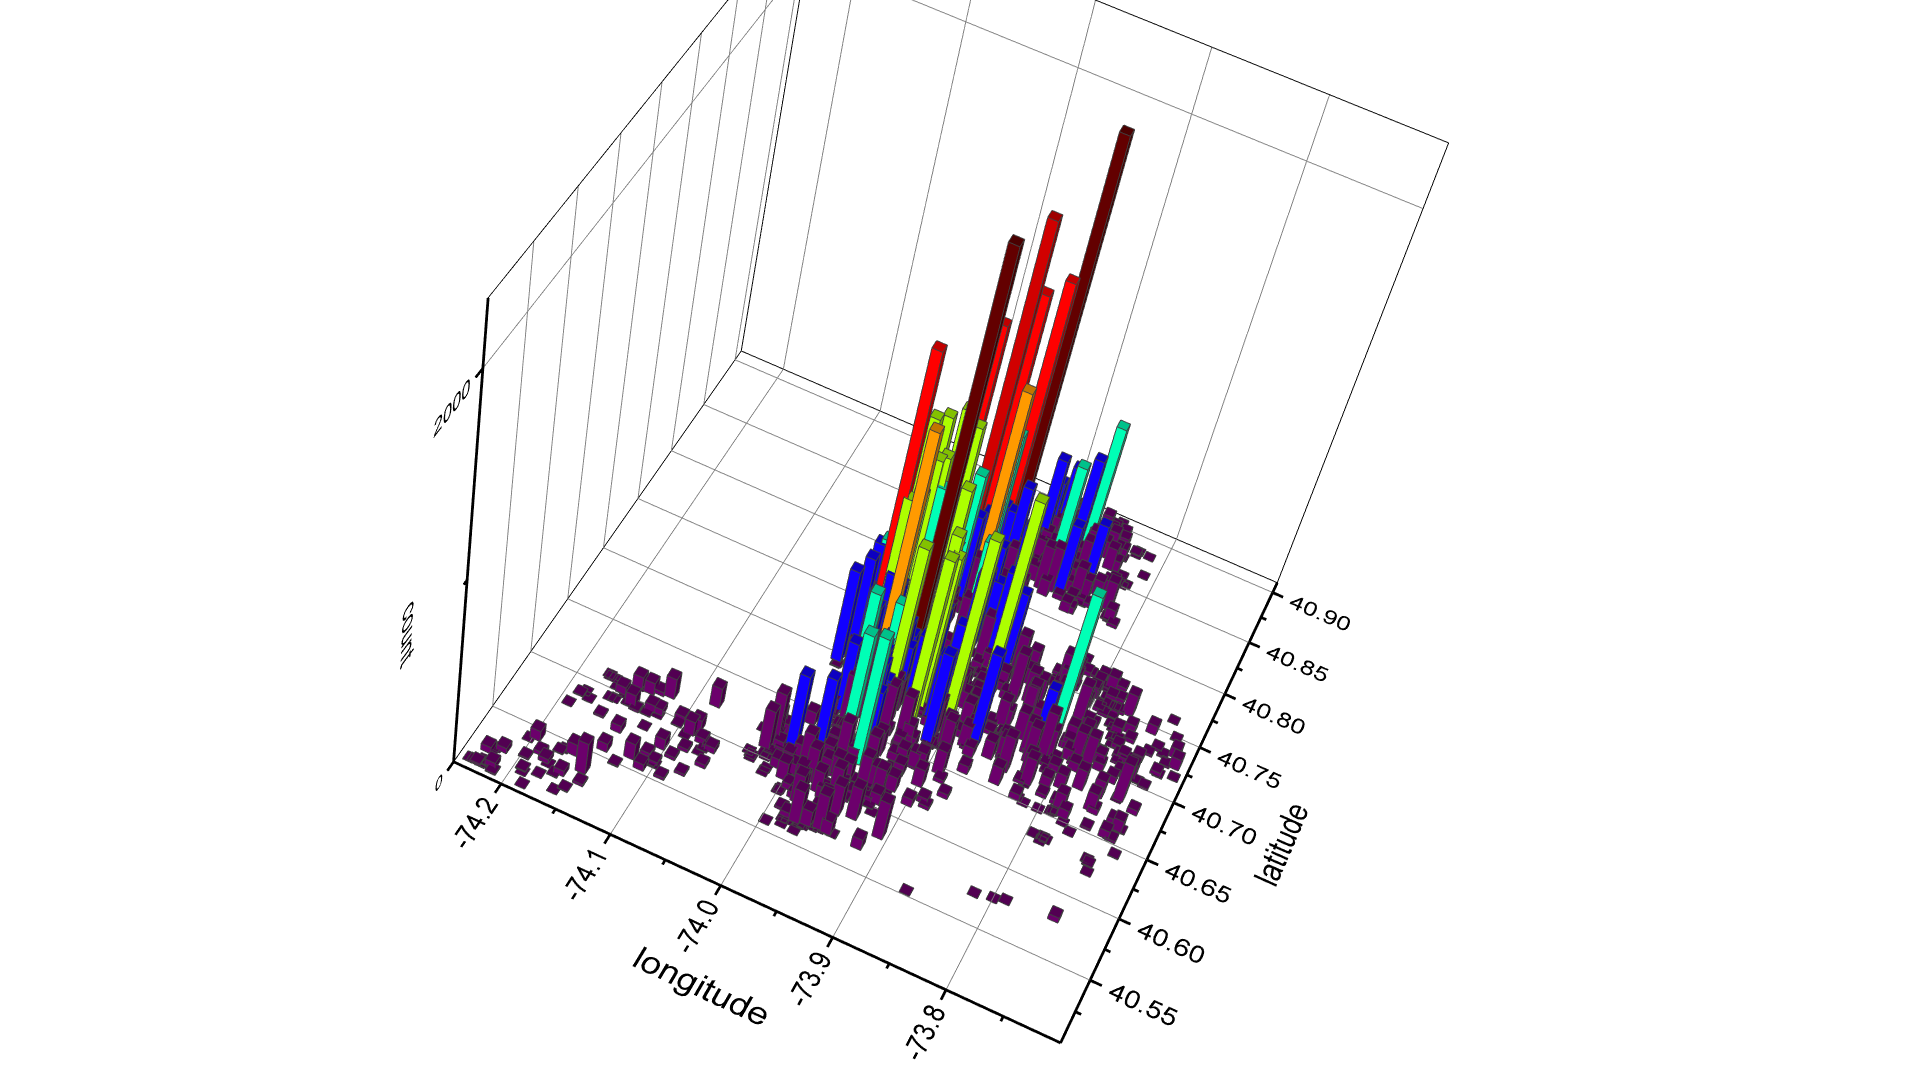
\includegraphics[scale = 0.2]{noise.png}
\end{minipage}
}
\subfigure[非法停车投诉]{
\begin{minipage}[t]{0.4\linewidth}
\centering
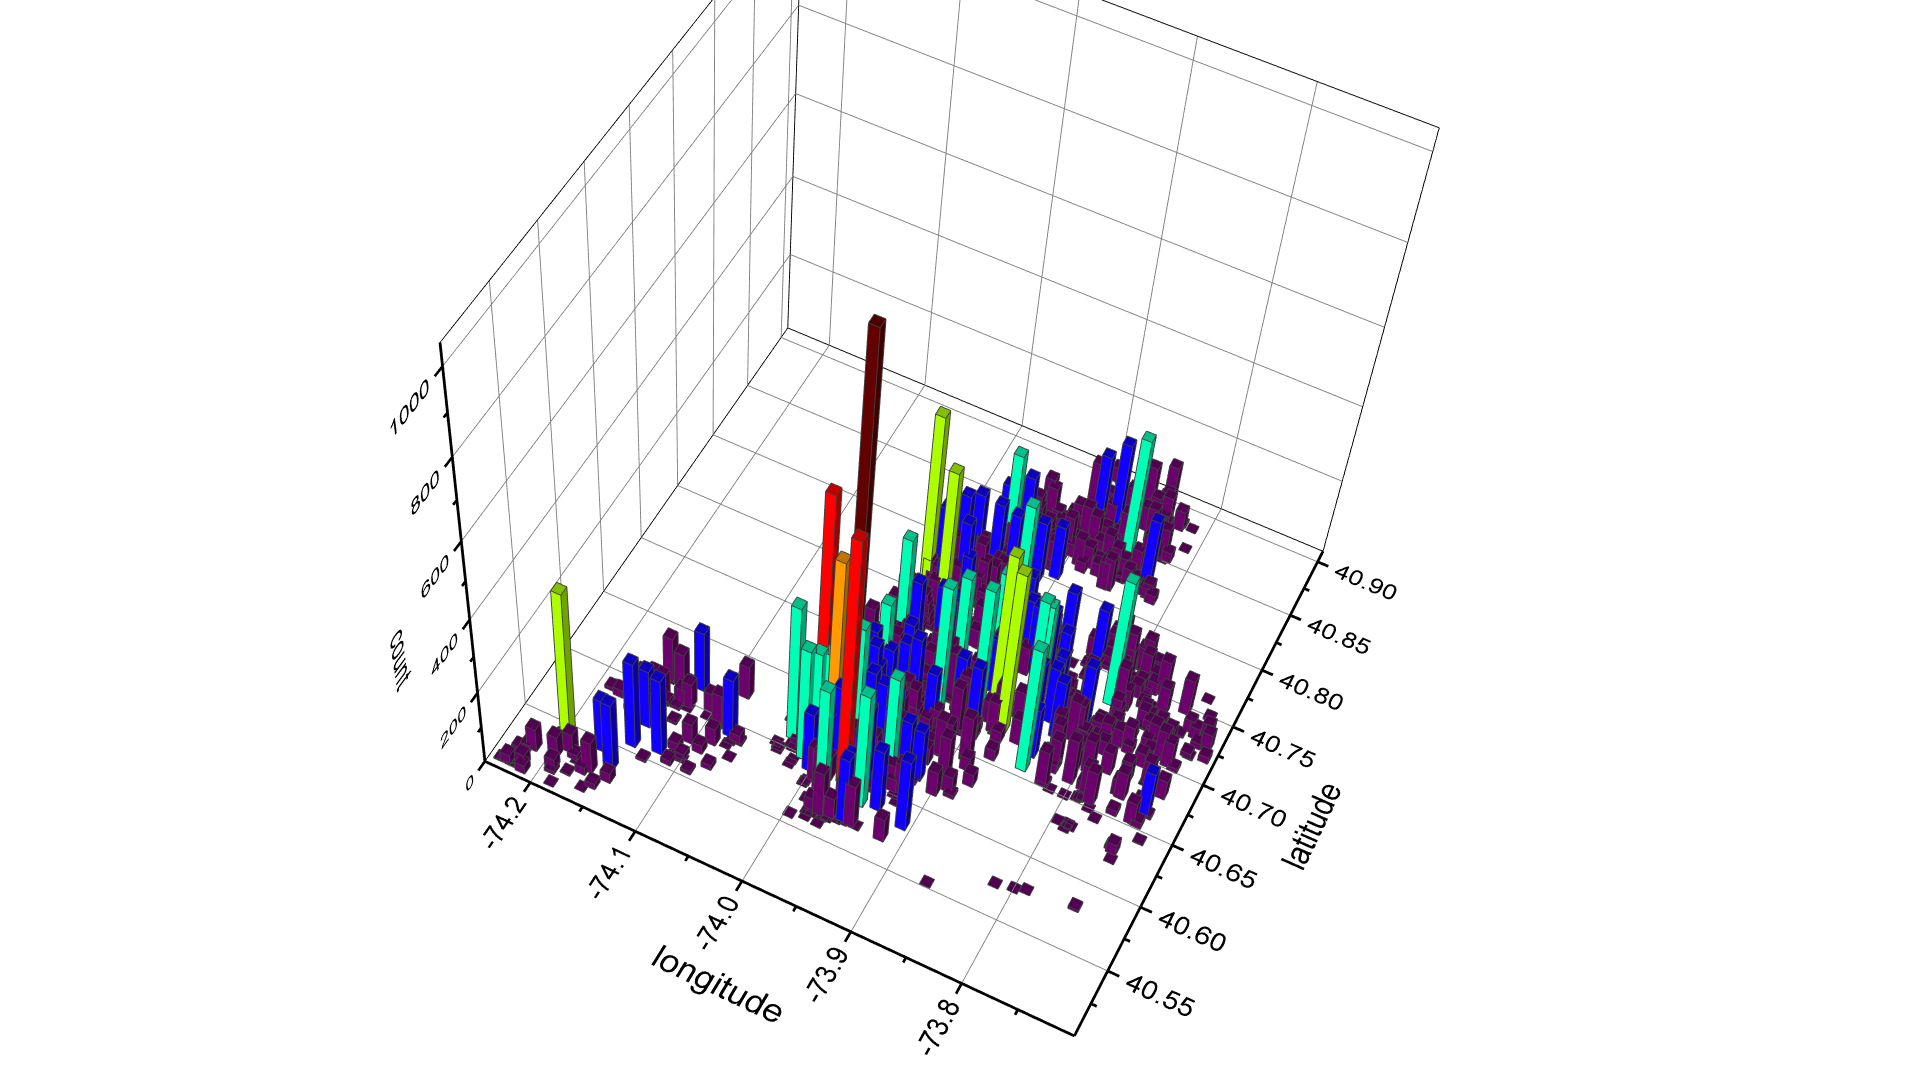
\includegraphics[scale = 0.2]{illegal.png}
\end{minipage}
}
\subfigure[堵塞投诉]{
\begin{minipage}[t]{0.4\linewidth}
\centering
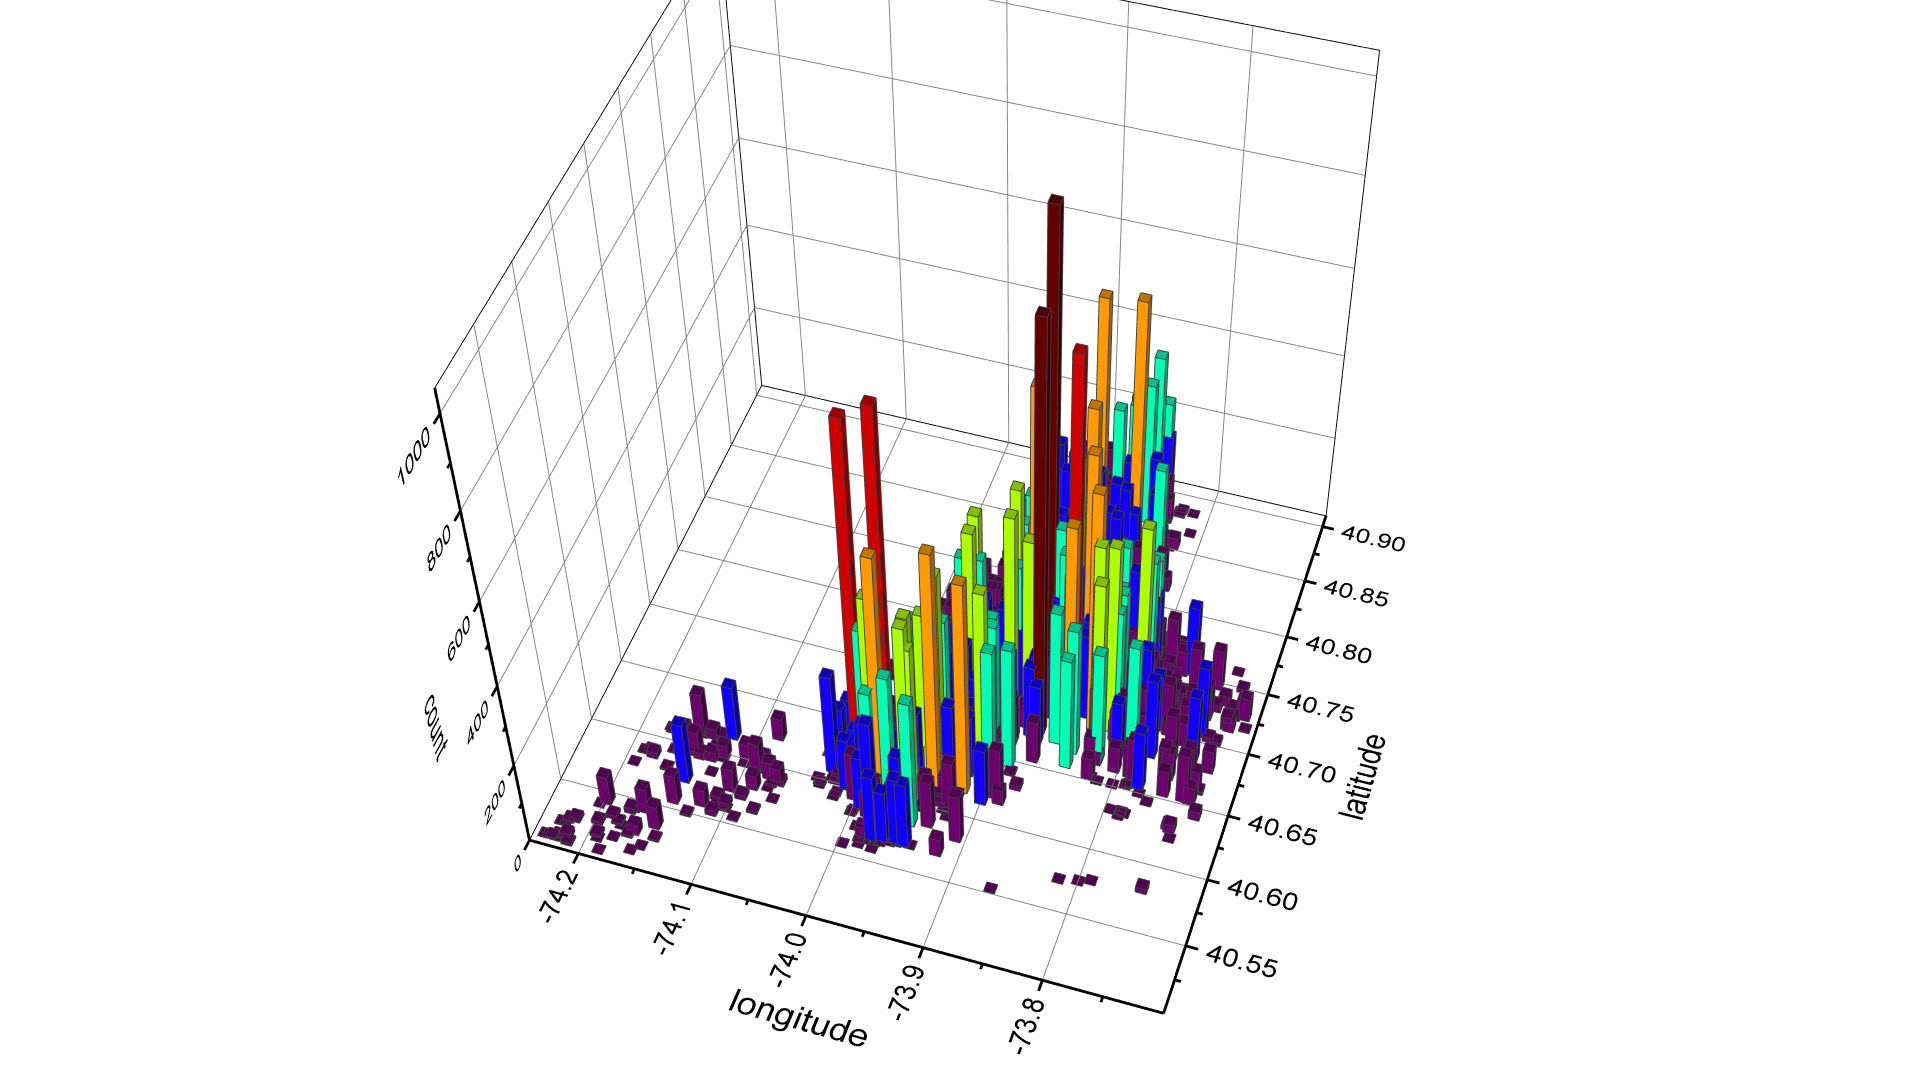
\includegraphics[scale = 0.2]{blocked.png}
\end{minipage}
}
\subfigure[其他类型]{
\begin{minipage}[t]{0.4\linewidth}
\centering
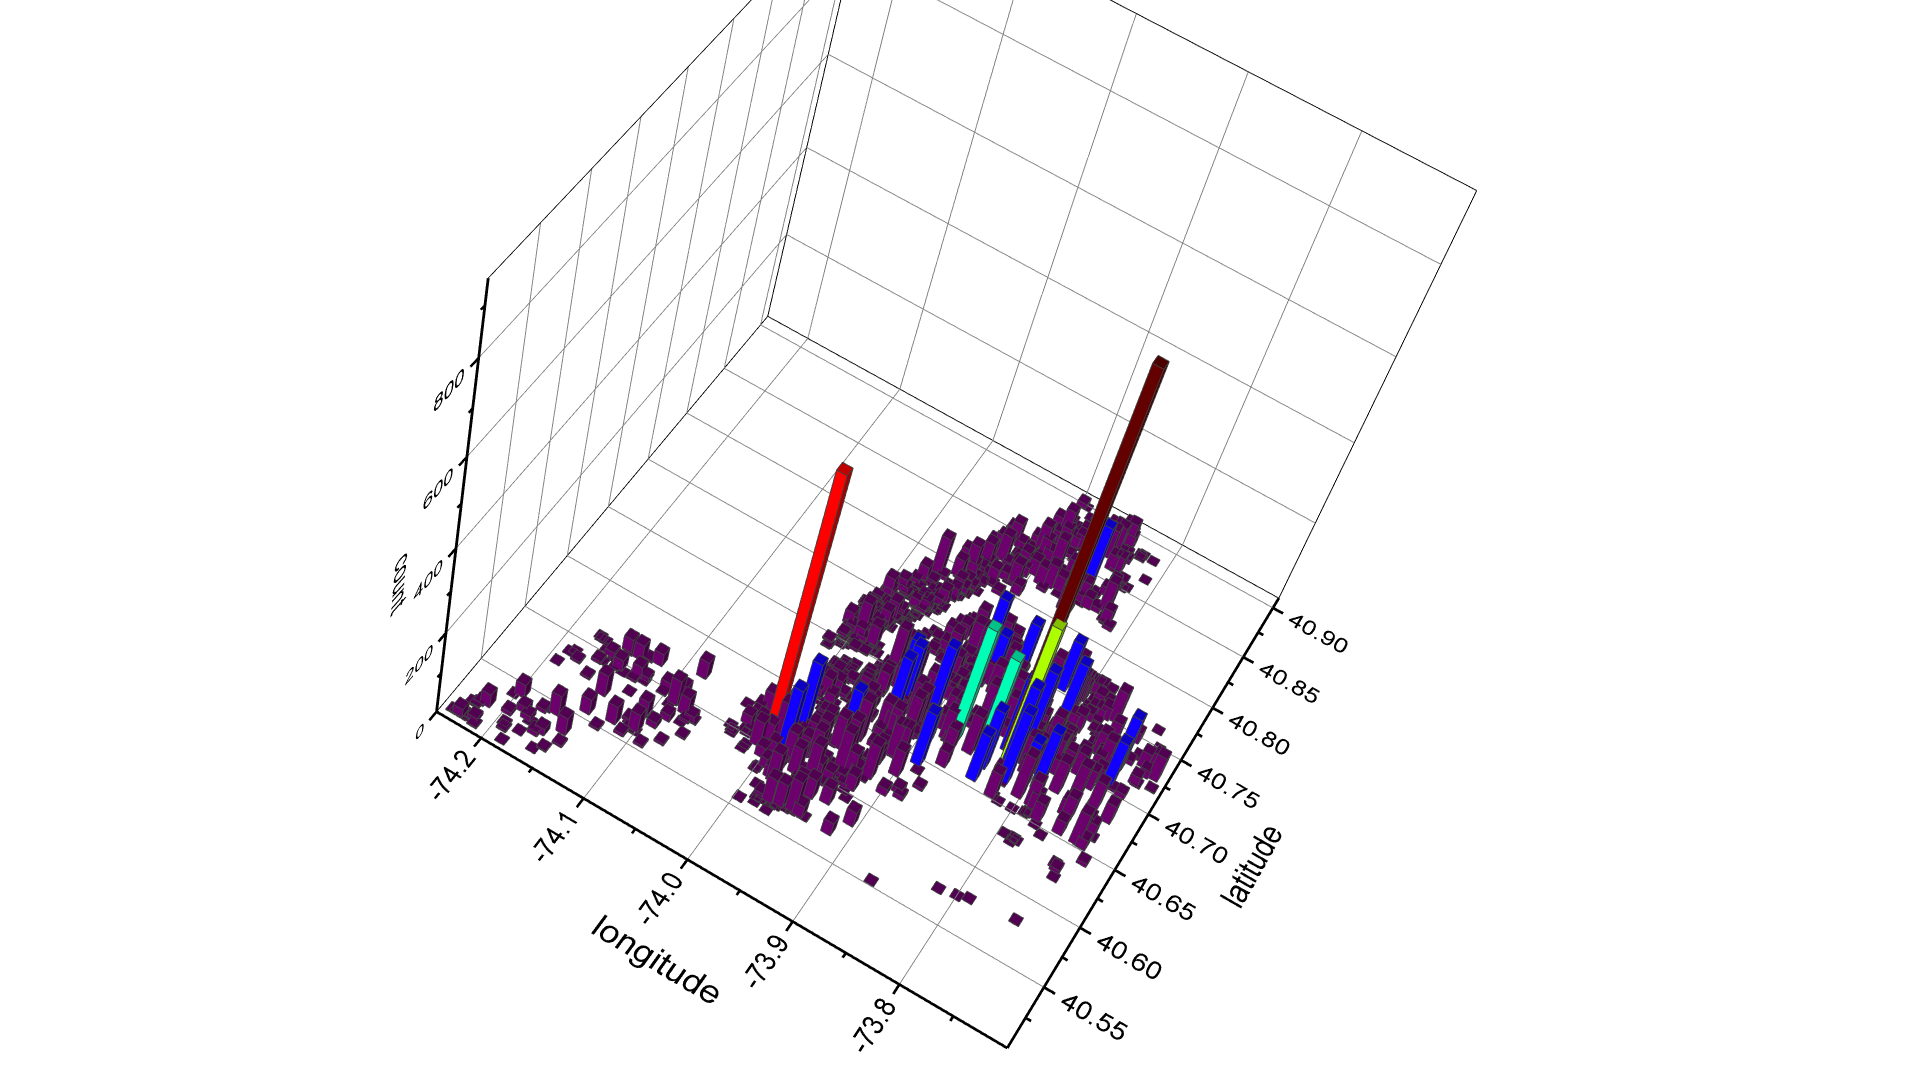
\includegraphics[scale = 0.2]{others.png}
\end{minipage}
}
\centering
\caption{311投诉}
\label{311}
\end{figure}

\begin{figure}[ht]
\label{ds1-1}
\centering
\subfigure[]{
\begin{minipage}[t]{0.4\linewidth}
\centering
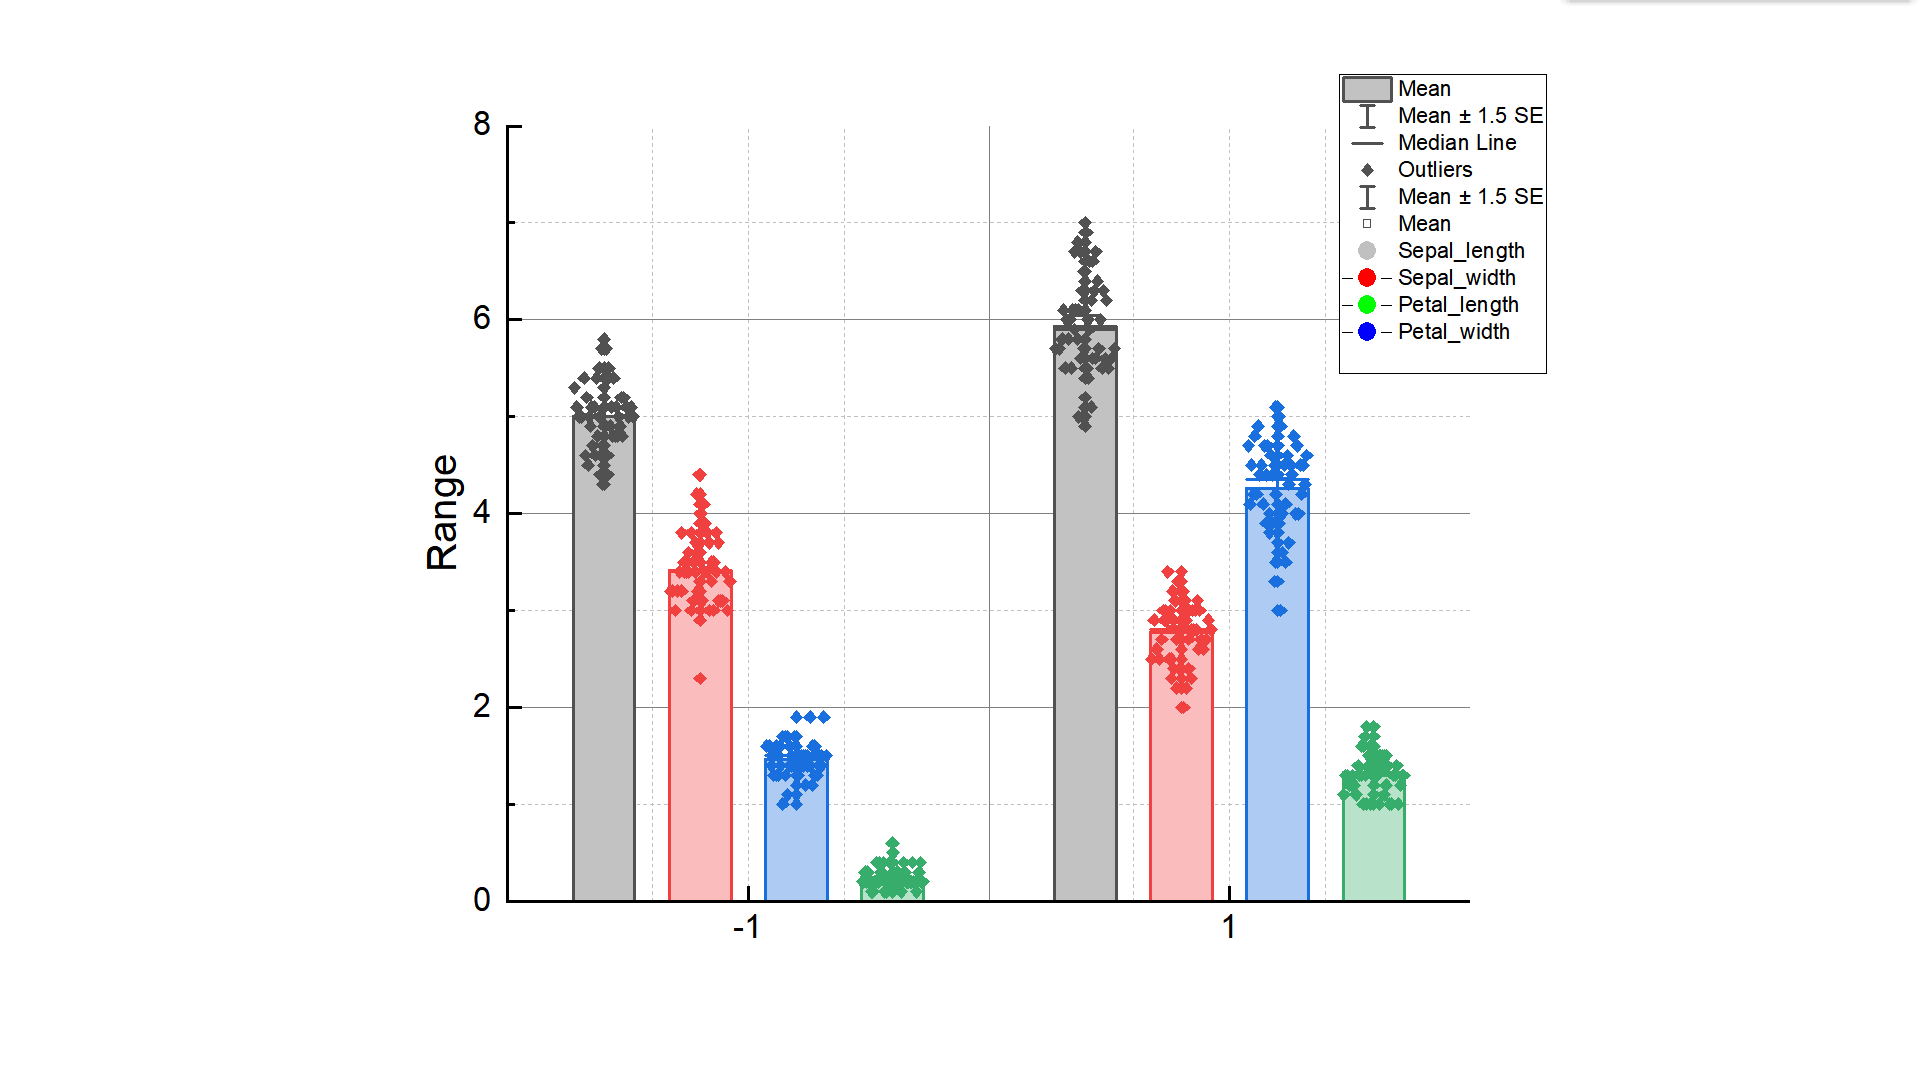
\includegraphics[scale = 0.2]{ds1-1.png}
\end{minipage}
}
\subfigure[]{
\begin{minipage}[t]{0.4\linewidth}
\centering
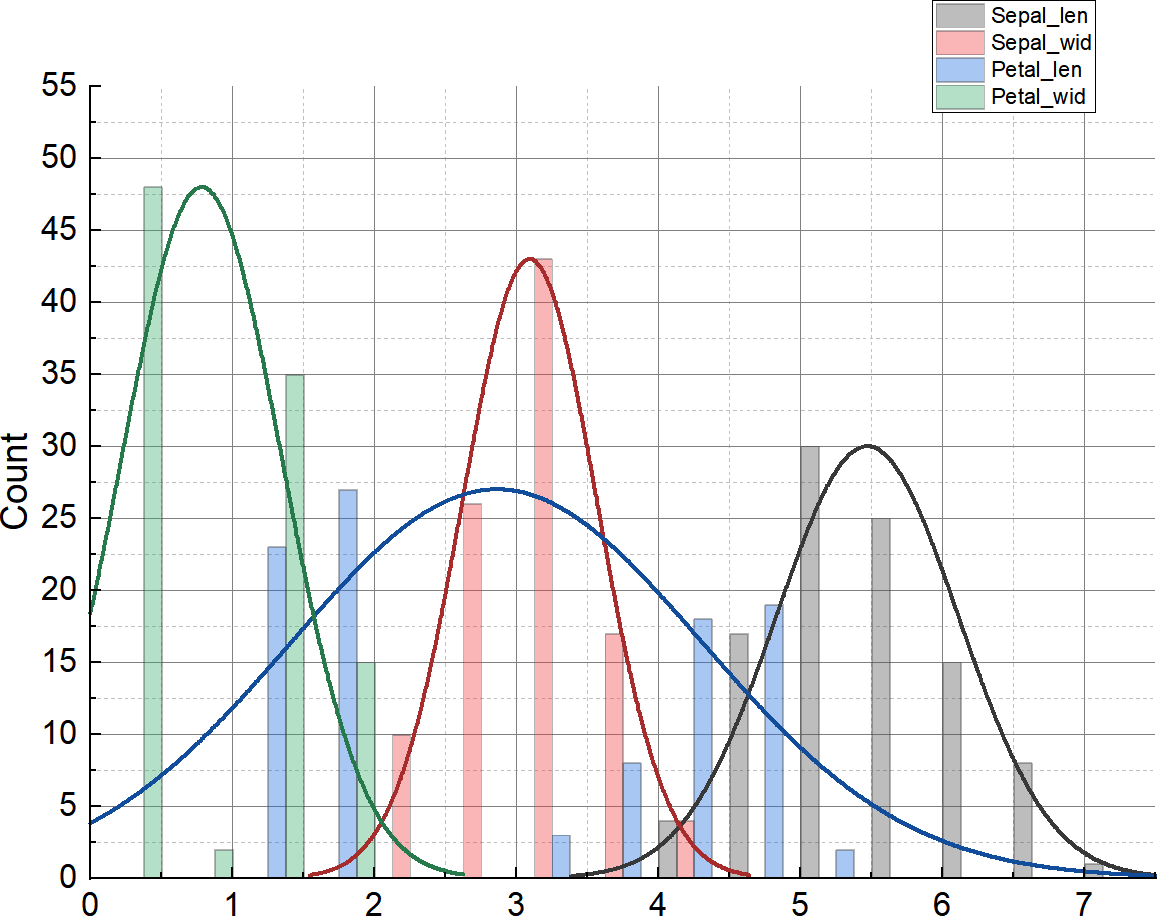
\includegraphics[scale = 0.2]{ds1-2.png}
\end{minipage}
}
\caption{}
\end{figure}

\end{CJK}
\end{document}
